\documentclass{sigchi}

\toappear{Submitted for review.} % replace this with the actual copyright strip when preparing the camera-ready
\pagenumbering{arabic} % comment this out when preparing the camera-ready

\usepackage{balance} % balance columns on last page
\usepackage{booktabs} % use booktabs instead of ugly regular tables
\usepackage{graphicx}
\RequirePackage[l2tabu, orthodox]{nag}
\usepackage{microtype}
\usepackage{url} % consider a nicer typeface (like Inconsolata) for URLs

%added for table
\usepackage{multirow}
\usepackage[table,xcdraw]{xcolor}
\usepackage{adjustbox}
\usepackage{amsmath}

\def\pprw{8.5in}
\def\pprh{11in}
\special{papersize=\pprw,\pprh}
\setlength{\paperwidth}{\pprw}
\setlength{\paperheight}{\pprh}
\setlength{\pdfpagewidth}{\pprw}
\setlength{\pdfpageheight}{\pprh}

\interfootnotelinepenalty=10000 % split footnotes are ugly
\tolerance=400 % reduce how often words stick out into columns at the expense of word spacing

\graphicspath{{figures/}} % put all your figures in this folder

\begin{document}

\title{Rewind: Automatically Generated\\Digital Memories from Mobile Geolocation Data}

\numberofauthors{3} % change this for additional authors
\author{
  \alignauthor {~}\\
    \affaddr{~}\\
    \affaddr{~}\\
    \email{~}\\
}

% DO NOT UNCOMMENT! submission is supposed to be anonymized
%\author{
% \alignauthor Eda Celen\\
%    \affaddr{Computer Science}\\
%    \affaddr{Brown University}\\
%    \email{edabingol@gmail.com}\\
% \alignauthor Phuc Anh D. Tran\\
%    \affaddr{Computer Science}\\
%    \affaddr{Brown University}\\
%    \email{pdtran@cs.brown.edu}\\
% \alignauthor Jeff Huang\\
%    \affaddr{Computer Science}\\
%    \affaddr{Brown University}\\
%    \email{uist@jeffhuang.com}\\ % Don't use my brown email here. Email addresses here get spam.
%}

\maketitle


% heather - add more results in here since we have more to report. Probably cut down image manipulation?
\begin{abstract}
We introduce \textit{Rewind}, a system that assists in the recall of semantic and episodic memory by automatically recreating interactive sceneries of past trips. \textit{Rewind} uses historical geolocation data to generate egocentric videos of earlier experiences from publicly-available street side images. Since the effectiveness of memory cues is determined by their level of integration with the target memory, images used in \textit{Rewind} are manipulated to incorporate time-of-day, seasonal and weather information, thereby creating more faithful representation of the original experience. Users can interactively go back and forth in time by scrubbing over the video. Together, the composed \textit{Rewind} videos offer users a window into past travels. We report the results of a user study with eighteen participants conducted to collect location data over two weeks. Trips taken in groups were more likely to be recalled using \textit{Rewind} videos than trips taken alone. \textit{Rewind} also serves as an experiment of the extreme scenario where users can freely roam and experience the world, keeping their mobile devices in their pockets, and still preserve believable representations that capture the past.
\end{abstract}

\keywords{
Digital memories, geolocation, streetside images, travel.
}

% Obviously replace this with the appropriate classification.
% Check if the CHI format asks for using the 2012 ACM classification instead of the 1998 one.
\category{H.5.m.}{Information Interfaces and Presentation (e.g. HCI)}{Miscellaneous}

\section{Introduction}

Capturing a memory is a fundamental part of human nature. Not long ago, we chronicled significant moments in our lives through journals and diaries, to be filled at the end of the day. Then came the cameras, to take with us when we expected a memorable moment. Now smartphone cameras are always nearby, ready for an opportunity to capture both the spectacular and the mundane. This paper introduces Rewind, a prototype of the next evolution in digital memories: nothing to prepare or take out, just rewind and replay a trip from the past.
 
While a camera or camcorder can explicitly capture a snapshot of an interesting moment, that one snapshot is only a small part of an experience, made even smaller when traveling. In fact, most travel experience happens in transit: the perfectly cloudy stroll from the Eiffel Tower to the Louvre, the sound of dry gravel crackling under bus tires traversing up to Machu Picchu or monsoon rains drumming on all the tin roofs of Hanoi, and even the flight over the Florida Keys on the way to the sun-bathed Caribbean islands. A simple photograph lacks this type of context.
 
Geolocation data that can be automatically tracked and logged on a smartphone can be used to recreate context: to look up the weather at each moment, retrieve street side photos (e.g. from Google Street View) at every step, and compute the mode of transportation (e.g., \cite{zheng2008learning}) and nearby geographical features. The Rewind system takes those cues and manipulates the conditions of retrieved photos to re-imagine what a person saw at some past point in time. The sequences of visuals are stitched together into an interface that allows users to directly manipulate the point in time being shown by scrubbing back and forth (Figure~\ref{fig:scrubbing}). So all a person has to do is enable location tracking on their mobile device to later rewind and re-experience a past trip.

\begin{figure}
   \centering
     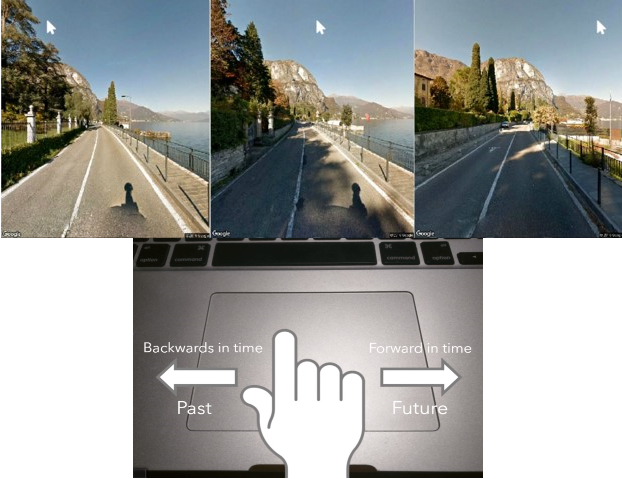
\includegraphics[width=1\linewidth]{scroll}
     \caption{Users move the stitched-together sequences of images forward and backward in time by scrubbing their pointer.}
     \label{fig:scrubbing}
\end{figure}

Rewind applies a framework for exploring fundamental questions about the human experience. Normally, it is difficult to ask someone about parts of their past that they do not entirely remember, because they do not remember what they do not remember.
% Note from Jeff: I'm not a fan of this example (that I commented out) because Rewinds don't recreate pictures of you either. Photos are actually much better at doing this.
% If you ask someone about a picture of themselves from ten years ago and they do not remember that particular point in time, there are no steps for re-remembering.
Using timestamped location data, we investigate whether a more realistic and contextual digital memory can help remind users of times from the past. Perhaps these Rewinds, sequence of images moving back and forth, can even help the forgetful recover past experiences. This could be done for people who are already tracking their location intentionally (using a smartphone app like Moves or GPSLogger), or for the many people for whom location tracking has been enabled by default on Android phones.

Through Rewind, we investigate what makes memories memorable, believable, and desirable. Participants in a two-week study looked at their own Rewinds and assessed which trips or places were more memorable, whether the Rewinds felt believable as their own memories, which memories they desired to preserve, and in this process, helped us gain a sense of what Rewinds are beyond static photographs. But not all memories are equally desirable. Through our study, we discovered not only what factors contribute to making a trip or place more memorable, but whether these are memories worth preserving. Are there aspects of a route that make a person want to review or relive a trip?
 
The two main contributions of our work are: 1) the design and implementation of the system for generating Rewinds, and 2) findings from a two-week user study where participants review Rewinds to describe what makes them memorable, believable, and desirable.

\section{Related Work}
% heather - trips vs locations -> (define) semantic memory vs episodic memory - check references, relate to some work done by SenseCam perhaps?
% cut down GPS usage
\subsection{Digital Memories}
Rewind is guided by literature about mediated memories, which provides a theoretical underpinning behind how the Rewind experience is constructed. \textit{Mediated Memories in the Digital Age} offers inspiration informing the relationship between experiences and memories \cite{van2007mediated}. van Dijck notes, ``Remembering is vital to our well being, because without autobiographical memories we would have no sense of past or future, and we would lack any sense of continuity'' (pg. 3). Rewind aims to give the user this sense of continuity in a time segment which has a past and future. By picking a start and end location from a particular trip and generating a Rewind between these points, the user relives their memories in a continuous manner. Similarly in his famous seminal paper \textit{As we may think}, Vannevar Bush described \textit{memex}, the envisioned machinery to store infinite information and to allow free, collective access through``associative trails'', giving mankind the ability of``...forgetting the manifold things he does not need to have immediately at hand, with some assurance that he can find them again if they prove important''. Rewind in its most ambitious form, perhaps strives to become a potential counterpart of \textit{memex} for retrieving, and sharing of autobiographical memories of one’s sensory experiences about past visits.

van Dijck also states that ``Our memories organize themselves according to our actual or perceived participation in a (temporal) collectivity---a group vacation, a school class, a family, a generation---and recall tends to lean on a sense of belonging or sharing rather than on a relocation in real time or space'' (pg. 9). Relating to the concept of organization, our user study explores whether traveling alone or with others affects the remembrance and the value of a past trip. 

Our study also extends the current state of knowledge about memory landmarks, although in a visual form. Horvitz et al. discuss how some events are particularly able to guide recall \cite{horvitz2004learning}. For example, these may be meetings with a high probability that the user will be in attendance. In Rewind, we seek to discover whether certain characteristics of a location, such as it being frequently visited or far away from home, serve as memory landmarks in the same way. 

Previous work has been done in moving memory from the realm of the mind to digital space in the field of psychology. Legge et al. experiment with the Method of Loci, a mnemonic technique where one stores things-to-be-remembered in a mental construction of a familiar place, called a memory palace \cite{legge2012building}. The stored remembrances can be retrieved by going through the memory palace in one's mind. Legge et al. found that virtual environments performed as well as mental environments for remembering serial lists. Rewind takes digital location-based memories and enhances them further for a virtual environment. Our user study explores whether Rewinds as a digital mnemonic device can perform as well as their predecessor, the photo.

Perhaps the most similar system to Rewind is Google+ Stories \cite{googlestories}, where the location coordinates are extracted from a user's photos and overlaid on a map. The interactivity of the photo album allows users to feel like they are going through a trip, rather than simply a series of photographs. Rewind takes this a step further by testing the extreme case where no personal photos are available, and everything is generated purely from timestamped location data that has been collected automatically.

\subsection{Location History}
A project that also leverages location data to capture the essence of a trip is by Thudt et al., who discuss the creation and investigation into the challenges and limits of visual mementos \cite{thudt2016visual}. The authors define visual mementos as ``visualizations of personally relevant data for the purpose of reminiscing, and sharing of life experiences.'' They present one implementation example of visual mementos that involves GPS location histories. This common goal of providing a way for people to reminisce about their trips reinforces the purpose of Rewind. Another reinforcement can be found in the way that their system is enhanced with geotagged photos from Flickr. The three main challenges presented in Thudt et al.'s paper are: 1) evoking familiarity, 2) expressing subjectivity, and 3) obscuring sensitive data. The authors attempt to address those challenges in the tool they built, called Visits, and their findings from the case study show that there is benefit to the visualization of personal mementos. Rewind builds on their work by breaking a trip down into smaller sequences and recreating the visual experience, whereas Visits relies on a more traditional top-down map view and timeline.

Another project by de Silva and Aizawa has also relied on geolocation data to provide a visual examination of interested traveling routes by linking geo-tagging metadata with online imageries, specifically Google Street View images \cite{deSilva:2009:RMT:1631272.1631414}. The authors proposed a sketch-based interface that would perform spatial and temporal queries on line drawings specified by the users. Rewind resembles this interactive system, in a way that the reconstructed sceneries are of a careful mapping results from geolocation data and Google Street View images. However, Rewind differs in that the mapping is finalized with geolocation data provided by users tracked using smartphones. This means that Rewind serves more of a getaway for recalling episodic memory rather than reviewing a potential travelling itinerary, aiming to provide a mechanism for reminiscence and sharing of past experience while exploring users' behavioral patterns. Moreover, the reconstruction techniques used in Rewind would differentiate the same retrieved image with various temporal cues such as changes in seasons; yet the immediate results from the temporal queries suggested by de Silva and Aizawa have not been fully revealed. 

Other research has used location history not to create a new interface for the user, but for other applications. Neuhaus's UrbanDiary project \cite{neuhaus2010urbandiary} uses GPS devices to create and visualize ``personal tracks'' as well as collective tracks for a city. These personal tracks are created using data from time and location tracking for each trip by each individual. The researchers focused on comparing the different visualization techniques used to portray data from a two-month study involved twenty participants wearing GPS devices. Using geotagged images from Flickr, Becker et al.'s work has shown that movement trajactories in metropolian areas tend to converge at Points of Interests(POIs) \cite{Becker2015}. The data from these studies show each person's location data can be used as a unique fingerprint. This supports the idea that location data can be used to help people recreate their individual travel experiences, for purposes of reminiscing and even sharing. In a similar vein, Cranshaw et al. \cite{cranshaw2012livehoods} recognize the ability for collective location data to understand the social patterns in a city. That everyone travels their own path, and this is part of their identity, is a core theme in Rewind.

Further work in location-based user behavior has been done by Leshed et al. to see how users interpret and interact with spaces differently when using in-car GPS navigation \cite{leshed2008car}. They found that ``the GPS disconnects the drivers from the external environment.'' As a result of the drivers' disengagement with their surroundings, ``the process of interpreting the world, adding value to it, and turning space into place is reduced to a certain extent and drivers remain detached from the indifferent environments that surround them.'' Since Rewind touches on the topic of travel, it also inherently deals with car travel and GPS. We imagine that regular GPS users will interact with Rewinds differently.

A common thing to do with location history data is to develop a visualization of it. Larsen et al. use a spiral chart for a user to see the continuity of their locations, where days are put around the spiral \cite{larsen2013qs}. This visualization allows users to explore and discover patterns in their daily lives. An early implementation of Visits by Thudt et al. focuses on the map and timeline views of location, interleaving them together \cite{thudt2013visits}. In their visualization, users can move from location to location using their pointer, which at the same time moves back and forth in time. This partially inspired the scrubbing technique in Rewind of traveling back and forth in time by scrubbing left and right, at the same time changing the image of what was seen at that time.
 
Finally, as location reveals where a person was at certain times, and is often a comprehensive view of someone's routes, there are substantial privacy concerns for this type of data. Not only can it reveal a person's home location, but it can also be used to forecast where they might be at a certain time in the future, or where they might not be. Lindqvist et al. \cite{lindqvist2011m} investigate the motivation behind sharing location data, and find that people are sensitive to privacy especially for places frequently visited (like their home). Tang et al. study the feeds of location histories meant for sharing, and discover that users desire different levels of details to be shared with other depending on their relationship with that person \cite{tang2011understanding}. The location itself is often not the concern, but that it is associated with an activity, which is the more sensitive variable. Users also unanimously disliked sharing time-based location, as it was too privacy-invasive. This informed our design of Rewind, where the generated experiences will not specify exactly the location, nor the time it represents. Users have the option to explicitly share a Rewind with another person after reviewing it themselves.

\begin{figure}[h]
   \centering
     \includegraphics[width=1\linewidth]{Rewind-Sample-Grid}
     \caption{Rewinds are generated by stitching together Google Street View images of consecutive points on a given route, which are manipulated to match the conditions from the past point in time. Rewinds are played from left to right to simulate a person on the move.}
     \label{fig:rewinds}
\end{figure}

\section{The Rewind System}

%%%%%%%%%%%%%%%%%%%%%%%%%%%%%%%%%%%%%%%%%%%%%%%%%%%%%%%%%%%%%%%%%%%%%%%%%%%%%%%%%%%%%%%%%%%%%%%%%%%%%%%%%%%%%%%%%%%%%%%%%%%%%%%%
% heather - depth of processing, retrival cues, uniqueness of encoding - Rewind ----> retrival cues
% http://www.psych.utoronto.ca/Neuropsychologylab/PDF/Depth%20of%20processing,%20retrieval%20cues,%20and.pdf
% go into introduction?
% come back to this section if time allows.
%%%%%%%%%%%%%%%%%%%%%%%%%%%%%%%%%%%%%%%%%%%%%%%%%%%%%%%%%%%%%%%%%%%%%%%%%%%%%%%%%%%%%%%%%%%%%%%%%%%%%%%%%%%%%%%%%%%%%%%%%%%%%%%%
\textit{Rewind} recreates the visual sensation of travelling down past routes using raw Google Location History data retrieved from location-tracking apps, including the default tracking behavior on Android phones. Differing from previously studied hyperlapse creation techniques, such as the studies by Kopft et al. and Joshi et al \cite{Kopf:2014:FHV:2601097.2601195, Joshi:2015:RHC:2809654.2766954}, \textit{Rewind} does not require any cinematic archives from the users, and it is computationally lightweight. \textit{Rewind} inputs geolocation data, maps out tracked trajectories, and outputs photo-video pairs with Google Street View images (although other street side photo services may be used). The sceneries in each photo-video pair are customized for each user based on times of the day, meteorological conditions and seasonal changes when the route was taken, providing users with multi-dimensional temporal cues. The current version of \textit{Rewind} is a open-sourced, web-based application implemented with Google Maps API and third-party JavaScript libraries, and therefore does not transfer sensitive user data nor store them. \textit{Rewind} can be accessed at [anonymized: url to rewind].  %\ref{fig:flowchart}

% \begin{figure}
%      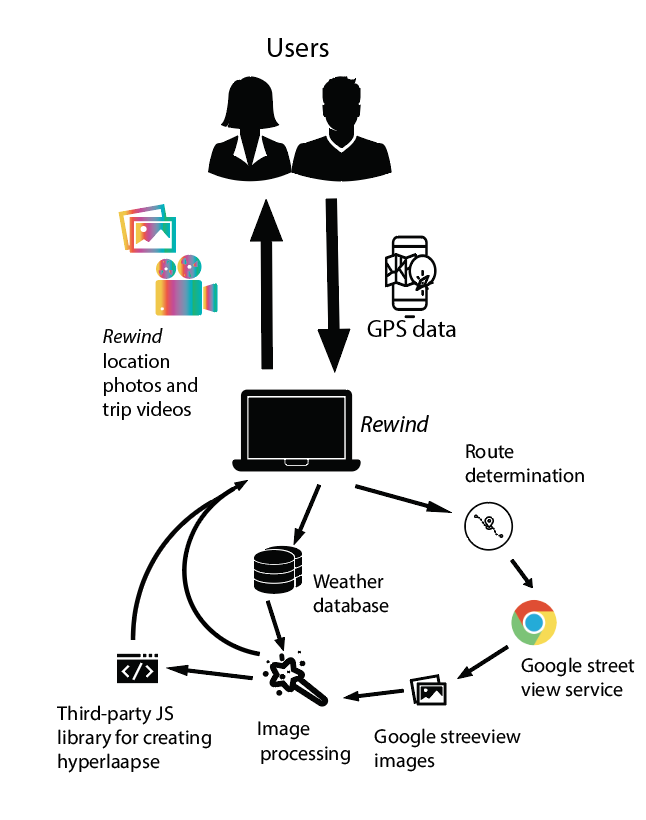
\includegraphics[width=1\linewidth]{Rewind-flowchart}
%      \caption{Plantation is classified using HSV color space, and the HSV values were adjusted to reflect seasonal changes}
%      \label{fig:flowchart}
% \end{figure}

% heather - add determination of home?
\subsection{Route Selection}
A user's geolocation tracking data includes latitude and longitude coordinates, and timestamps of when the user was at given coordinates. \textit{Rewind} expects JSON formatted data, and is also compatible with other location-based formats such as GPX. Rewind generates location points for the user, using smart filtering based on visit frequencies to decrease the data noise and diversify the locations shown to the user.

When the user loads their location data into Rewind, it filters out location coordinates with < 200 meter accuracy, and a location frequency map is generated by counting the number of times each location appears in history. In order to minimize the minor coordinate variations and to identify close coordinate pair records, only the first 3 decimal digits of coordinates are used when counting the number of appearances. The location with the highest number of visits is marked as user's home. Rewind then uses the Haversine formula to calculate the individual distance between all given locations and the user's home, attaching the distance data to the location.

\begin{figure*}
	\centering
	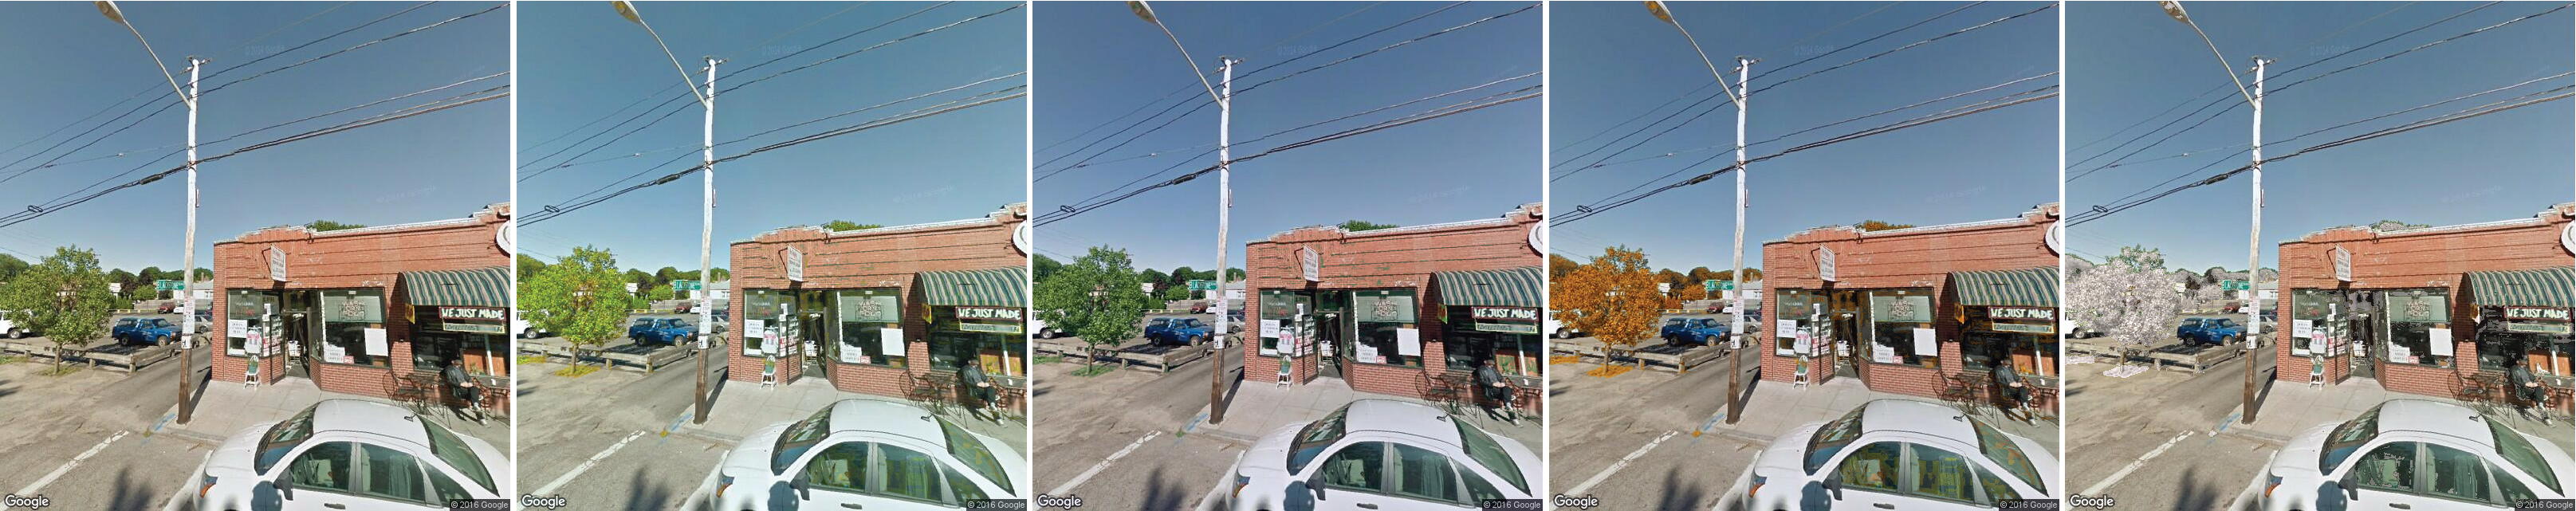
\includegraphics[width=\textwidth]{Rewind-seasons2}
	\caption{Plantation is classified using HSV color space, and the HSV values were adjusted to reflect seasonal changes}
	\label{fig:season}
\end{figure*}


\begin{figure*}
	\centering
	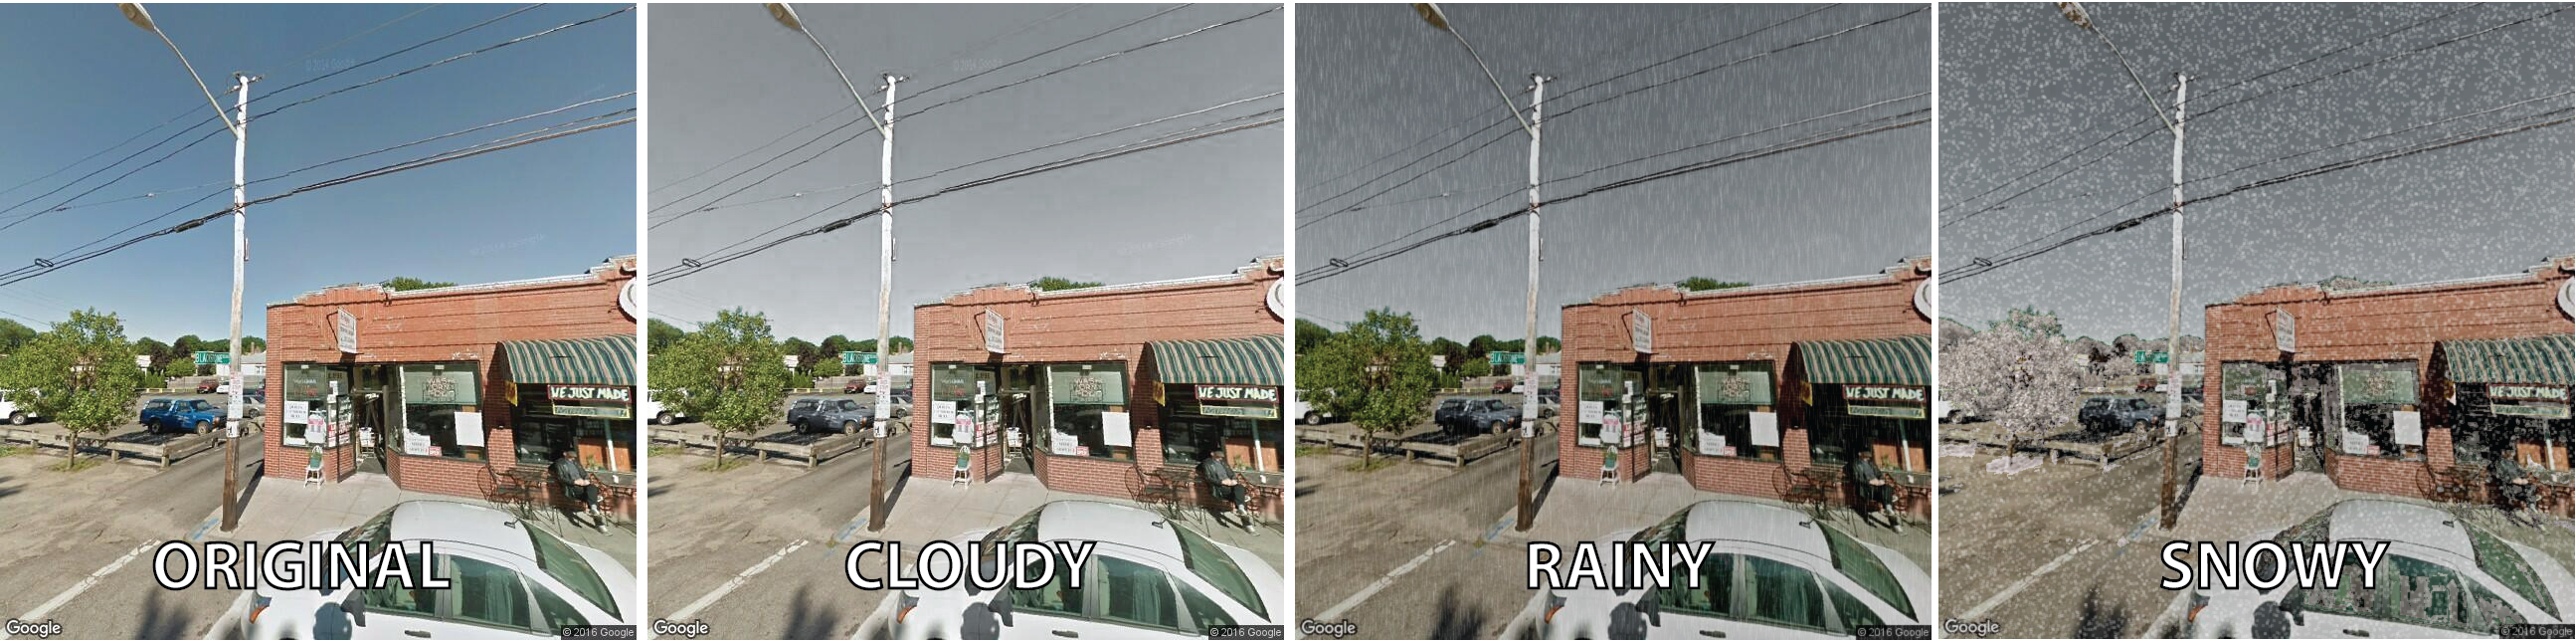
\includegraphics[width=\textwidth]{Rewind-weather}
	\caption{Meterological attributes are depicted using JavaScript canvas painting and animation}
	\label{fig:weather}
\end{figure*}

\begin{figure}
	\centering
	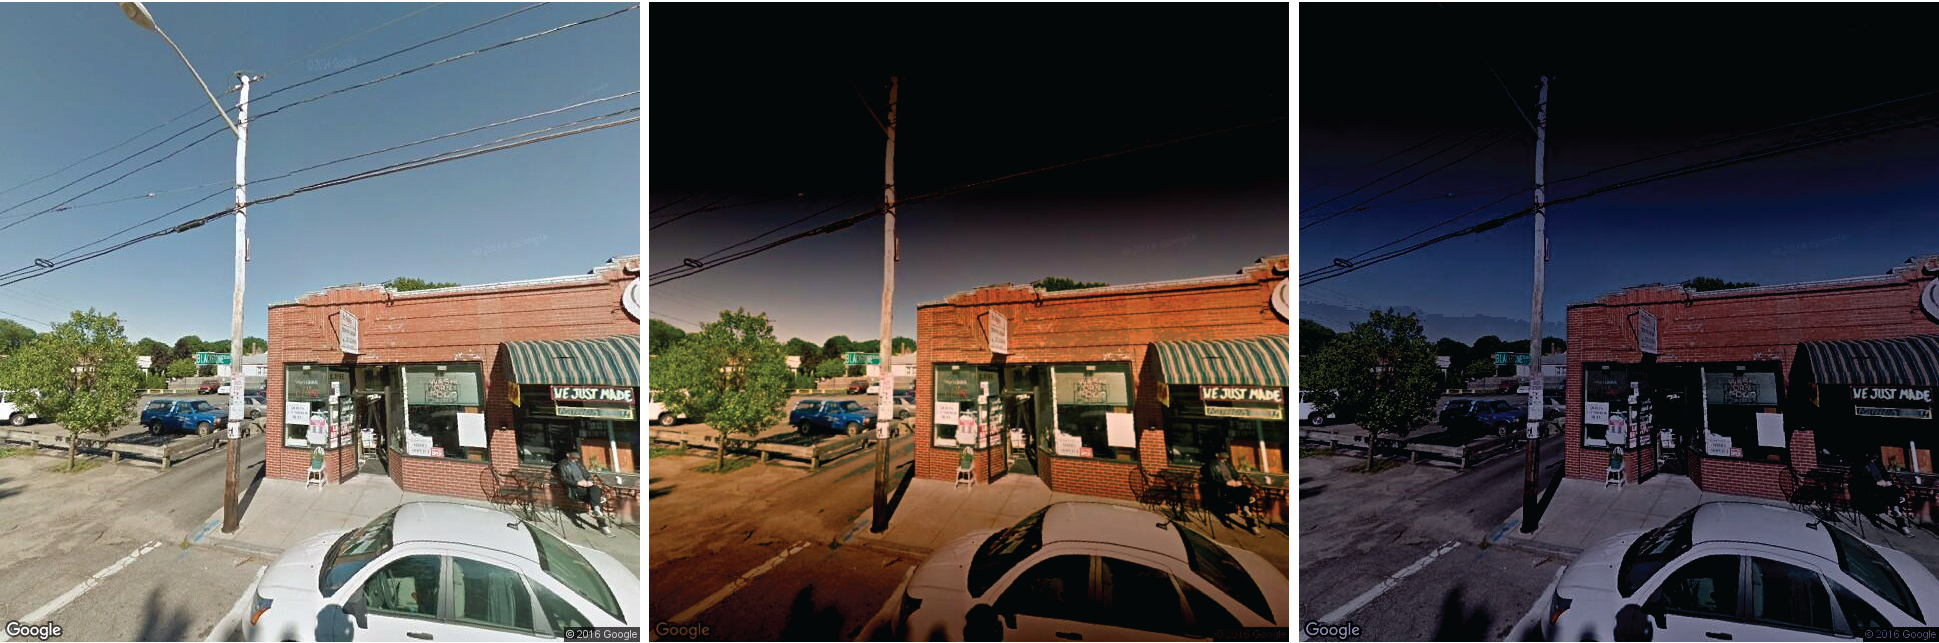
\includegraphics[width=1\linewidth]{Rewind-time_of_day2}
	\caption{Per-pixel change is applied based on classified region}
	\label{fig:timeofday}
\end{figure}

\subsection{Sequence Creation}
Each video recollection created by \textit{Rewind} is composed of two hundred Google Street View image sequences of the chosen route being stitched together using StreetViewSequence \cite{streetviewsequence}. Each incoming Google Street View image has been retrieved with the same dimensions (640 px by 640 px) with similar spatial orientation (FOV, pitch and heading values).

Since environmental characteristics, such as meteorological attributes, of images retrieved using Google Street View Static Image API are not directly exposed nor adjustable, it is hard to conclude if the retrieved images would correctly reflect the timely and ambient properties at the time when the user undertook the path. To compensate for this, pixel-wise adjustment was applied on each Google Street View image to better convey time-specific messages including times of the day, seasonal variances and meteorological specifics. Previous work done by \cite{laffont2014transient,shih2013data} have successfully reconstructed images with varying diurnal and seasonal cycles, yet it would be computationally expensive to replicate the proposed techniques in real-time on large sets of images. Considering each \textit{Rewind} sequence of images would contain two hundred frames, this process would take many hours per route, and it would be challenging to incorporate a large training dataset into the rendering pipeline. Due to the timing constraint, Rewind instead adopts a simplified approach of color space mapping for object segmentation and color adjustment, with the facilitation of CamanJS \cite{caman}.

As the Google Street View images of a given route have been retrieved with the same dimensional parameters and optical orientation, locational and spatial information of each image is largely similar (ex. the sky normally resides in the upper 1/3 of the image, but could occupy more than 1/2 of the image at times). Thus sky and ground regions could be approximated by generalizing the observed geographical information of the incoming images. Each pixel was first converted from RGB representation into HSV color space. For seasonal changes, a range of HSV values was estimated for plantation classification and those HSV values that fell within the range were adjusted for desired seasonal effects. Each HSV value was then converted back to RGB color space for JavaScript canvas painting (Figure~\ref{fig:season}). Similarly, for creating nightly effects such as sunset and evening scenes, sky colors were modified using the same technique. In addition, two linear brightness and saturation filters were applied locally and globally (Figure~\ref{fig:timeofday}). As an example of creating the evening scene, the incoming Google Street View images were segmented into three major areas: 1) Approximated sky region 2) Non-sky region in the approximated sky region 3) Approximated Ground region. RGB values of each pixel were down-scaled based on the region the pixel is classified in. 

For meteorological conditions, a NoSQL database populated by data collected from the National Oceanic and Atmospheric Administration (NOAA) weather stations was used for weather lookup (for the study, only data from [anonymized: our state/province] was loaded). Sky colors were adjusted again using the technique mentioned previously for overcast, rainy and snowy sky. For determined rainy and snowy periods of time, an animated precipitation layer was overlaid on the sequence of images and accompanied by corresponding audio effects to emulate the weather conditions exposed by the data (Figure~\ref{fig:weather}). Note that in the user study reported in this paper, an earlier version of the image manipulation was used, which adjusted whole-image color attributes.

% (Jeff): I think this is an unnecessary detail for this paper
%For the user study, Rewind displayed one image at a time on the browser, along with an identifier code. The first character in the code is a letter from the group \{R,M,L\}, followed by an integer number. The first character represents the visit frequency of the location shown in the image: R for randomly selected, M for points selected from the most frequently visited locations, and L for points selected from the least frequently visited locations. The integer that follows denotes the distance in meters between a user's home and the given location "as the crow flies." 

% heather - perhaps giving this part a new title? 
\subsection{User Interaction}
Users can click on the images to load the accompanying ``trip'' videos (stitched sequence of images), or Rewinds. The purpose of the Rewinds is to help users remember locations and trips.
% Note from Jeff: Cut this sentence because I don't understand it. What's a ``corresponding image''?
% Rewinds are composed of locations visited on the same date as the Rewind's corresponding image.
When the user loads a Rewind, all the locations the user visited on that day are gathered and sorted, after which a route is mapped between the locations using the Google Maps API.
% Note from Jeff: Reader doesn't know what StreetviewSequence is, and probably does not need to
% This route data is passed to StreetviewSequence to generate Rewinds by stitching together images. For each point on a given route, StreetviewSequence
For each point in the route, Rewind determines the appropriate pitch and heading values to get the correct portion of the panorama. Those values are sent to Google Street View along with the necessary geolocation data to retrieve images that will be stitched together to make the Rewind.

In order to account for time of day and season changes,
% StreetviewSequence library is modified to allow Rewind to
Rewind intercepts and manipulate each frame of the trip video, similar to the manipulations applied to the 10 location images. Once all the images within a trip are gathered from Google Street View and processed with CamanJS, users can play Rewinds in a loop, or scrub forward and backward over the video to investigate individual images more closely.

\section{User Study}
\subsection{Research Questions}
% heather - is "digital memory" the right phrase for describing Rewind? Isn't rewind a medium for providing the cues to retrieve exisiting memories rather than creating new memories?
% talk about both within-subject and between-subject comparisons 
% within-subject -> memorability -> efficacy of semantic memory retrival vs episodic memory retrival -> video is better for both sementic and episodic
% between-subject -> memorability -> what type of users benefit the most from episodic memory retrival using Rewind; what kind of trip is Rewind best at capturing - (least frequently visited trip? most frequently visited trip? trip that's far away from home?)
The Rewind system enables us to ask questions about people's attitudes and behaviors surrounding digital memories that were not possible to answer before due to the scarcity of comprehensive data about where a person has been. To understand what makes a digital memory meaningful to a person, we performed a within-subjects comparison of Rewinds and static photos. By comparing Rewinds to today's most prevalent form of digital memory media, we can distill what features make a Rewind meaningful and representative as a memory of a trip.

Our research questions examine the effectiveness of \textit{Rewind} videos through three virtues of a memory: memorability, believability, and desirability. % heather - do we need a reference for the three virtues?


% heather - I changed this part...
\begin{enumerate}
\item Memorability: How would \textit{Rewind} facilitate the retrival of semantic and episodic memory? What types of users are most likely to recall their memories using \textit{Rewind}?
\item Believability:  How accurate are \textit{Rewind} artifacts in the eyes of the users' ? 
\item Desirability: What factors are inherent to users' decisions in preserving artifacts created by \textit{Rewind}?
\end{enumerate}

% heather - where to put this part or do we need a summary like this at all?
%%%%%%%%%%%%%%%%%%%%%%%%%%%%%%%%%%%%%%%%%%%%%%%%%%%%%%%%%%%%%%%%%%%%%%%%%%%%%%%%%%%%%%%%
Our user study explored the following five metrics that could potentially influence the aforesaid three measurements of \textit{Rewind} vidoes. These five metrics are:
\begin{enumerate}
\item GPS usage: how self-identified regular GPS users and non-regular GPS users differ in their responses to \textit{Rewind} videos.
\item Traveler type: how self-identified frequent and non-frequent travelers report to the three measurements of \textit{Rewind} videos differently.
\item Companions: how traveling companionship and solitude affect users' viewpoints on \textit{Rewind} videos.
\item Distance: how traveling distances influence users' perceptions of \textit{Rewind} videos.
\item Visit frequency: how visit frequency of a particular place influences users' reporting on \textit{Rewind} videos.
\end{enumerate}
%%%%%%%%%%%%%%%%%%%%%%%%%%%%%%%%%%%%%%%%%%%%%%%%%%%%%%%%%%%%%%%%%%%%%%%%%%%%%%%%%%%%%%%%

\subsection{Participants}
To recruit a diverse local population, participants for the user study were recruited online through local forums (Craigslist classifieds and local Reddit communities). Offline, ads were posted in cafes and other small businesses in the the city. Of the 21 total participants, 13 were identified as men and 8 were identified as women, with age ranged from 20 to 50 years old. Participants were mainly local residents, with occupations including librarian, medical researcher, office worker, IT consultant, student, musician, and comedian.
% Jeff notes, comment this out because it's not remarkable
% A fifth of the participants were undergraduate or graduate students.

\subsection{Procedure}
Participants underwent a two-week tracking period followed by a mixed-methods user study which investigated the memorability, believability, and desirability of \textit{Rewind} artifacts produced from the two weeks of location data.

Study participation included a setup session for location tracking, at least twelve days of tracking, and a follow-up user study. At the location tracking setup, participants were asked to activate geolocation tracking on their mobile phones. Participants with Android devices used Google's built-in location reporting services for tracking. iPhone users downloaded the Google+ app to use the same service. Participants with devices incompatible with Google's location reporting services were provided with an older Android device that used the GPSLogger\footnote{\url{https://play.google.com/store/apps/details?id=com.mendhak.gpslogger&hl=en}} app for tracking. Participants were asked to keep their phone charged and on their person as much as possible for approximately two weeks, until they could come in for a final interview with the experimenters.

At the in-person interview, participants were shown a series of photos and accompanying Rewinds that represented the trips they took during the tracking period. The participant's geolocation data was trimmed to ensure that photos and Rewind videos were generated from data gathered no earlier than the past two weeks. Participants were shown ten photo-Rewind pairs in a semi-structured interview.  Of the ten pairs, five showed trips taken infrequently, three showed trips taken most frequently, and the remaining two were random. 

At the beginning of the study, participants were asked to identify their gender, whether they considered themselves a frequent traveler, and whether they tended to use GPS in places they were already familiar with.
Then, questions about the photos and Rewinds investigated their memorability, believability, and desirability.

%Participants who used GPS in familiar locations were considered regular GPS users, and participants who did not were considered non-regular GPS users.
For each photo-Rewind pair, the participant was first shown a photo of one of the locations found in their geolocation data. The participant was asked to answer the following questions about the photo: Do you remember this location? If so, can you name the street? Can you name what is around the location, such as buildings, landmarks, or other places? Would you want to keep this photo? Why or why not? Were you traveling alone? If you remember the location, is the photo accurate to your memory? Why or why not? What was different?

% heather - Rewind of the trip or Rewind video of the trip?
The participant was then shown a Rewind of the trip that they were on when the previous location was encountered. While the Rewind was playing, the participant could hover over the Rewind panel and scrub backwards and forwards horizontally through the images that composed the video. This allowed participants to ``walk through'' their memory at their own pace. The participant was asked the following questions while the Rewind played: Do you remember these locations? Do you remember this particular trip? Can you name some of the streets? Can you name what is around these locations, such as buildings, landmarks, or other places? Would you want to keep this video? Why or why not? Were you traveling alone? If you remember these locations, is the video accurate to your memory? Why or why not? What was different?

In addition to asking questions, we observed the users as they examined their generated Rewinds, since they could passively watch the Rewind or actively scrub through the individual images that made up the Rewind. The user study took between 30 minutes to an hour for each participant, and participants were compensated \$30 for their time at the end of the study.

% heather - ...that they did not carry the device on their person. - grammatical error?
Data from three participants was not included in the results of this study. One of the participants' data points consisted of only one location. The participant used a mobile device provided by the study, so it is likely that they did not carry the device on their person. Another participant did not complete the in-person interview portion of the user study due to health and scheduling reasons. The last participant only collected three days of data because they had their phone replaced during the tracking period, and did not reactivate Google's location reporting services on their new device. This participant completed the in-person interview portion of the user study, but we did not include the data gathered during this participant's session in the results.


% heather - need to be rephrased perhaps? Should we give a high level summary of all the relationships we've found? More analysis to be done for photo vs. videos, another table?
% semantic vs episodic memory
% mention distance categories in the beginning (up up up) + everything else 
\section{Findings}
The findings of our user study center on the participants’ relationship to the Rewinds generated from their location data. We focus on the participants’ judgments of their Rewinds’ memorability, believability, and desirability in comparison to their judgments of the photos paired with the Rewinds. We also discuss the participants' interactions with and reactions to their Rewinds. The results use data from the user studies conducted with 12 men and 6 women. Half of the participants identified themselves as frequent travelers. Additionally, half of the participants were regular GPS users, that is people who used GPS even in locations already familiar to them.

\subsection{Within-subject study}
\subsubsection{Semantic Memory} 
Within-subject comparison in our study reveals that participants are significantly better at recalling semantic memory of a particular location with \textit{Rewind} videos than with static street-view images, $\chi^2(1, N=356) = 96.987$, $p <.01$. When being presented with a street-side image retrieved based on their location data, participants were able to recognize places visited 50\% of the time; yet recognition rate of locations reached 97\% when participants started playing accompanied \textit{Rewind} video, with a significant increase of 47\%. It is perhaps not too surprising as cinematic media like \textit{Rewind} video would provide users with more contextual meanings and retrival cues for semantic processing, as three participants (P4, P6 and P10) have once expressed their contentment after watching \textit{Rewind} videos by claiming ``I recognize the photo now!'' when their initial attempts with static images recognition were fruitless. 

%
\subsubsection{Episodic Memory}
It could possibly be inferred that participants are likely to benefit more from \textit{Rewind} videos than static street-view images at recalling episodic memory. Although participants were not explicitly asked about trip rememberance when presented with static images as opposed to what they were asked after watchiing \textit{Rewind} videos, location rememberance from static images may serve as an upper-bound estimation of how much an individual could recall about a particular trip; since if participants fail to form any cognitive association with the locations depicted in the images, it is very unlikely that they would be able to associate target itineraries with the locations shown. Thus, it is perhaps safe to presume that location rememberance with images bounds above the maximum likelihood of trip rememberance with the same images presented to the participants, and we used location rememberance from image recognition as an upper-limit gauge against trip rememberance from \textit{Rewind} videos thereafter.

% h - add another table, only abt memorability tho
% explain distance groups in the beginning
% where is home? need to explain this part in system?
Using the aforementioned presumption, our study examined effects of \textit{Rewind} videos on episodic processing in metric-specific groups, as well as the performance overall. Our study shows that comparing to static street-view images, recollection of event-driven memories using \textit{Rewind} videos is significantly improved for trips taken that were 100 - 1,000 km (62 - 620 miles) away from home by 50\%, $\chi^2(1, N=20) = 3.215$, $p <.05$; and for trips that were least frequently taken by about 20\%, $\chi^2(1, N=161) = 5.977$, $p <.01$. Our study also suggested that GPS users would benefit more from \textit{Rewind}, even though the difference was mildly significant by an increase about 15\%, $\chi^2(1, N=118) = 2.145$, $p = .0715 (<.1)$. 
% h - prob explain this a little bit more

One plausible explanation of the improvement may be inherent to the encoding of episodic memory in the first place. As suggested by the levels-of-processing theory(ref), encoding efficacy is heavily dependent on the levels to which stimuli are being actively or passively processed. Not surprisingly, superficial mental engagement would produce weaker, and less enduring cognitive representation which would demand more contextually accurate and abundant cues for memory triggery, and vice versa. Oftentimes, the cognitive representation resulted from shallow processing may not even be retrievable at all as it is simply not available for retrieval.  As previously described, both of the trips revealed in our results, those that were taken farthest away from home and those that were least frequently taken, may not be special enough to engage deep memory encoding nor often enough to reinforce incidental remembrance. This means that it would be more difficult for participants to recall these trips if the provided cues are not effective enough. Since \textit{Rewind} videos provide richer and more contextually meaningful cues than static street-side images, it is reasonable that \textit{Rewind} significantly outperforms plain images as suggested by our statistical analysis. While being asked about location and trip rememberance on one of his least frequently taken routes, P7 was not able to identify the location from the static image at first; yet he recognized the trip from \textit{Rewind} video as ``one street (in the video) helps me (him) remember". 
%The Effects of Divided Attention on Encoding and Retrieval Processes in Human Memory 
% http://www2.psych.ubc.ca/~pgraf/Psy583Readings/Craik%20et%20al%201996.pdf
% Craik et al. 1996

The extent to which attention is dedicated while taking a trip may be another possible explanation for the observed improvement using Rewinds. This is perhaps particularly applicable to explain why participants who were self-identified regular GPS users tend to benefit more from Rewinds with episodic memory recalling. Laboratory work done by Craik et al. 1996 (ref) has demonstrated that the encoding of memory is more effective under full-attention conditions than divided-attention conditions.  This means that regular GPS users, who are often directed step-by-step on how to navigate through their environments, may be less likely to engage their attention while taking their routes, leading to less available cognitive representation for retrieval. P3, a self-identified regular GPS user who had 30\% recalling rate using static images and 80\% trip remembrance rate using Rewinds said ``I really don't pay attention to my surroundings when I'm driving. (I am) Focused (focused) on GPS and road"  Under this circumstance, it is almost certain that Rewinds would provide a more successful access to episodic memory as it provides more spatial-temporal cues for memory retrieval, by not only adjusting image attributes to reflect timely and weather changes, but also mimicing the motions of the users when they travel down a particular path. 

It may appear to be puzzling that participants seem to recall less about specifics of their trips from \textit{Rewind} videos compared to static images when they traveled alone, with a significant decrease around 40\%, $\chi^2(1, N=168) = 33.831$, $p <.01$; when the trips were most frequently taken, with a significant decrease of 20\%, $\chi^2(1, N=161) = 5.977$, $p <.01$; and when the trips taken were 10 - 100 meters (33 - 328 feet) away from home, with a mildly significant decrease of 50\%, $\chi^2(1, N=16) = 2.25$, $p <.1$. 


\subsubsection{Belivability and Desirability}
Although not statistically significant, 

\subsection{Between-subject study}


%%UPDATE BOTH TABLES AND ADD ONE MORE%%%
%%%%%%%%%%%percentage to decimal
\begin{table*}[t]
	\centering
	\caption{My caption}
	\small
	\label{within-subject-table}
	\begin{tabular}{c|c|c|c|c|c|c|c|c|}
		\cline{2-9}
		& \multicolumn{4}{c|}{Memorability} & \multicolumn{2}{c|}{Belivability} & \multicolumn{2}{c|}{Desirability} \\ \cline{2-9} 
		& \begin{tabular}[c]{@{}c@{}}video\\  location\end{tabular} & \multicolumn{2}{c|}{\begin{tabular}[c]{@{}c@{}}photo\\ location/trip\end{tabular}} & \begin{tabular}[c]{@{}c@{}}video\\ trip\end{tabular} & photo & video & photo & video \\ \hline
		\multicolumn{1}{|c|}{N} & 177 & \multicolumn{2}{c|}{179} & 177 & 86 & 128 & 179 & 177 \\ \hline
		\multicolumn{1}{|c|}{\%} & 96.61\% & \multicolumn{2}{c|}{49.72\%} & 53.67\% & 77.91\% & 79.69\% & 10.61\% & 14.69\% \\ \hline
		\multicolumn{1}{|c|}{p-val} & \multicolumn{2}{c|}{\begin{tabular}[c]{@{}c@{}}$\chi^2(1, 356) = 96.987$\\ p = 0.0001\end{tabular}} & \multicolumn{2}{c|}{\begin{tabular}[c]{@{}c@{}}$\chi^2(1, 356) = 0.41$\\ p = 0.2611\end{tabular}} & \multicolumn{2}{c|}{\begin{tabular}[c]{@{}c@{}}$\chi^2(1, 214) = 0.02$\\ p = 0.4434\end{tabular}} & \multicolumn{2}{c|}{\begin{tabular}[c]{@{}c@{}}$\chi^2(1, 356 ) = 0.995$\\ p = 0.1593\end{tabular}} \\ \hline
	\end{tabular}
\end{table*}
% 2nd table %%%%%%%%%%%%%%%%%%%%%%%%%%%%%%%%%%%%%%%%%%%

\begin{table*}[t]
	\centering
	\caption{My caption}
	\begin{adjustbox}{width=1\textwidth}
		\small
		\label{between-subject-table}
		\begin{tabular}{ccccccccccccccccc}
			\cline{4-17}
			\multicolumn{1}{c}{}                                 & \multicolumn{1}{c}{}                         & \multicolumn{1}{c|}{}      & \multicolumn{2}{c|}{GPS usage}                                                                                       & \multicolumn{2}{c|}{Traveller type}                                                                                  & \multicolumn{2}{c|}{Companions}                                                                                               & \multicolumn{6}{c|}{Distance}                                                                                                                                                                                                                                                                                                            & \multicolumn{2}{c|}{Visit frequency}                                                                                 \\ \cline{4-17} 
			\multicolumn{1}{c}{}                                 & \multicolumn{1}{c}{}                         & \multicolumn{1}{c|}{}      & \multicolumn{1}{c|}{GPS user}                             & \multicolumn{1}{c|}{non-GPS user}                        & \multicolumn{1}{c|}{Frequent}                             & \multicolumn{1}{c|}{Non-frequent}                        & \multicolumn{1}{c|}{Alone}                                     & \multicolumn{1}{c|}{Not alone}                              & \multicolumn{1}{c|}{0}                                & \multicolumn{1}{c|}{1}                               & \multicolumn{1}{c|}{2}                               & \multicolumn{1}{c|}{3}                               & \multicolumn{1}{c|}{4}                               & \multicolumn{1}{c|}{5}                               & \multicolumn{1}{c|}{Most}                                 & \multicolumn{1}{c|}{Least}                               \\ \hline
			\multicolumn{1}{|c|}{}                               & \multicolumn{1}{c|}{}                        & \multicolumn{1}{c|}{N}     & \multicolumn{1}{c|}{\cellcolor[HTML]{ACDDAA}60}           & \multicolumn{1}{c|}{\cellcolor[HTML]{ACDDAA}119}         & \multicolumn{1}{c|}{120}                                  & \multicolumn{1}{c|}{59}                                  & \multicolumn{1}{c|}{\cellcolor[HTML]{ACDDAA}74}                & \multicolumn{1}{c|}{\cellcolor[HTML]{ACDDAA}20}             & \multicolumn{1}{c|}{\cellcolor[HTML]{ACDDAA}5}        & \multicolumn{1}{c|}{\cellcolor[HTML]{ACDDAA}8}       & \multicolumn{1}{c|}{\cellcolor[HTML]{ACDDAA}18}      & \multicolumn{1}{c|}{\cellcolor[HTML]{ACDDAA}71}      & \multicolumn{1}{c|}{\cellcolor[HTML]{ACDDAA}64}      & \multicolumn{1}{c|}{\cellcolor[HTML]{ACDDAA}10}      & \multicolumn{1}{c|}{\cellcolor[HTML]{ACDDAA}47}           & \multicolumn{1}{c|}{\cellcolor[HTML]{ACDDAA}81}          \\ \cline{3-17} 
			\multicolumn{1}{|c|}{}                               & \multicolumn{1}{c|}{}                        & \multicolumn{1}{c|}{\%}  & \multicolumn{1}{c|}{\cellcolor[HTML]{ACDDAA}33.33\%}      & \multicolumn{1}{c|}{\cellcolor[HTML]{ACDDAA}57.98\%}     & \multicolumn{1}{c|}{50.83\%}                              & \multicolumn{1}{c|}{47.46\%}                             & \multicolumn{1}{c|}{\cellcolor[HTML]{ACDDAA}100.00\%}          & \multicolumn{1}{c|}{\cellcolor[HTML]{ACDDAA}55.00\%}        & \multicolumn{1}{c|}{\cellcolor[HTML]{ACDDAA}100.00\%} & \multicolumn{1}{c|}{\cellcolor[HTML]{ACDDAA}75.00\%} & \multicolumn{1}{c|}{\cellcolor[HTML]{ACDDAA}72.22\%} & \multicolumn{1}{c|}{\cellcolor[HTML]{ACDDAA}43.66\%} & \multicolumn{1}{c|}{\cellcolor[HTML]{ACDDAA}51.56\%} & \multicolumn{1}{c|}{\cellcolor[HTML]{ACDDAA}10.00\%} & \multicolumn{1}{c|}{\cellcolor[HTML]{ACDDAA}72.34\%}      & \multicolumn{1}{c|}{\cellcolor[HTML]{ACDDAA}35.80\%}     \\ \cline{3-17} 
			\multicolumn{1}{|c|}{}                               & \multicolumn{1}{c|}{\multirow{-3}{*}{\rotatebox{90}{photo}}} & \multicolumn{1}{l|}{p-val} & \multicolumn{2}{c|}{\cellcolor[HTML]{ACDDAA}\begin{tabular}[c]{@{}c@{}}$\chi^2(1, 179) = 8.734$\\ p =0.0016\end{tabular}}  & \multicolumn{2}{c|}{\begin{tabular}[c]{@{}c@{}}$\chi^2(1, 179) = 0.071$\\ p = 0.3953\end{tabular}}                         & \multicolumn{2}{c|}{\cellcolor[HTML]{ACDDAA}\begin{tabular}[c]{@{}c@{}}$\chi^2(1, 94) = 31.812$\\ p \textless0.0001\end{tabular}}  & \multicolumn{6}{c|}{\cellcolor[HTML]{ACDDAA}\begin{tabular}[c]{@{}c@{}}$\chi^2(5, 179 ) = 18.106$\\ p = 0.0028\end{tabular}}                                                                                                                                                                                                                   & \multicolumn{2}{c|}{\cellcolor[HTML]{ACDDAA}\begin{tabular}[c]{@{}c@{}}$\chi^2(1,128) = 14.458$\\ p = 0.0001\end{tabular}} \\ \cline{2-17} 
			\multicolumn{1}{|c|}{}                               & \multicolumn{1}{c|}{}                        & \multicolumn{1}{c|}{N}     & \multicolumn{1}{c|}{58}                                   & \multicolumn{1}{c|}{119}                                 & \multicolumn{1}{c|}{120}                                  & \multicolumn{1}{c|}{57}                                  & \multicolumn{1}{c|}{\cellcolor[HTML]{ACDDAA}94}                & \multicolumn{1}{c|}{\cellcolor[HTML]{ACDDAA}39}             & \multicolumn{1}{c|}{5}                                & \multicolumn{1}{c|}{8}                               & \multicolumn{1}{c|}{18}                              & \multicolumn{1}{c|}{71}                              & \multicolumn{1}{c|}{64}                              & \multicolumn{1}{c|}{10}                              & \multicolumn{1}{c|}{46}                                   & \multicolumn{1}{c|}{80}                                  \\ \cline{3-17} 
			\multicolumn{1}{|c|}{}                               & \multicolumn{1}{c|}{}                        & \multicolumn{1}{c|}{\%}  & \multicolumn{1}{c|}{48.28\%}                              & \multicolumn{1}{c|}{56.30\%}                             & \multicolumn{1}{c|}{53.33\%}                              & \multicolumn{1}{c|}{54.39\%}                             & \multicolumn{1}{c|}{\cellcolor[HTML]{ACDDAA}61.70\%}           & \multicolumn{1}{c|}{\cellcolor[HTML]{ACDDAA}89.74\%}        & \multicolumn{1}{c|}{60.00\%}                          & \multicolumn{1}{c|}{25.00\%}                         & \multicolumn{1}{c|}{55.56\%}                         & \multicolumn{1}{c|}{59.15\%}                         & \multicolumn{1}{c|}{50.00\%}                         & \multicolumn{1}{c|}{60.00\%}                         & \multicolumn{1}{c|}{52.17\%}                              & \multicolumn{1}{c|}{56.25\%}                             \\ \cline{3-17} 
			\multicolumn{1}{|c|}{\multirow{-6}{*}{\rotatebox{90}{Memorability}}} & \multicolumn{1}{c|}{\multirow{-3}{*}{\rotatebox{90}{video}}} & \multicolumn{1}{c|}{p-val} & \multicolumn{2}{c|}{\begin{tabular}[c]{@{}c@{}}$\chi^2(1, 177) = 0.713$\\ p =0.1992\end{tabular}}                          & \multicolumn{2}{c|}{\begin{tabular}[c]{@{}c@{}}$\chi^2(1, 179) = 0.017$\\ p = 0.4478\end{tabular}}                         & \multicolumn{2}{c|}{\cellcolor[HTML]{ACDDAA}\begin{tabular}[c]{@{}c@{}}$\chi^2(1,  133) = 9.016$\\ p = 0.0013\end{tabular}}        & \multicolumn{6}{c|}{\begin{tabular}[c]{@{}c@{}}$\chi^2(5, 177) = 4.754$\\ p = 0.4467\end{tabular}}                                                                                                                                                                                                                                             & \multicolumn{2}{c|}{\begin{tabular}[c]{@{}c@{}}$\chi^2(1, 126) = 0.066$\\ p =  0.3987\end{tabular}}                        \\ \hline
			\multicolumn{1}{|l|}{}                               & \multicolumn{1}{c|}{}                        & \multicolumn{1}{c|}{N}     & \multicolumn{1}{c|}{19}                                   & \multicolumn{1}{c|}{67}                                  & \multicolumn{1}{c|}{61}                                   & \multicolumn{1}{c|}{25}                                  & \multicolumn{1}{c|}{\cellcolor[HTML]{ACDDAA}71}                & \multicolumn{1}{c|}{\cellcolor[HTML]{ACDDAA}20}             & \multicolumn{1}{c|}{5}                                & \multicolumn{1}{c|}{5}                               & \multicolumn{1}{c|}{13}                              & \multicolumn{1}{c|}{30}                              & \multicolumn{1}{c|}{32}                              & \multicolumn{1}{c|}{1}                               & \multicolumn{1}{c|}{\cellcolor[HTML]{FFFFC7}34}           & \multicolumn{1}{c|}{\cellcolor[HTML]{FFFFC7}27}          \\ \cline{3-17} 
			\multicolumn{1}{|l|}{}                               & \multicolumn{1}{c|}{}                        & \multicolumn{1}{c|}{\%}  & \multicolumn{1}{c|}{68.42\%}                              & \multicolumn{1}{c|}{80.60\%}                             & \multicolumn{1}{c|}{77.05\%}                              & \multicolumn{1}{c|}{80.00\%}                             & \multicolumn{1}{c|}{\cellcolor[HTML]{ACDDAA}81.69\%}           & \multicolumn{1}{c|}{\cellcolor[HTML]{ACDDAA}25.00\%}        & \multicolumn{1}{c|}{80.00\%}                          & \multicolumn{1}{c|}{60.00\%}                         & \multicolumn{1}{c|}{69.23\%}                         & \multicolumn{1}{c|}{90.00\%}                         & \multicolumn{1}{c|}{75.00\%}                         & \multicolumn{1}{c|}{0.00\%}                          & \multicolumn{1}{c|}{\cellcolor[HTML]{FFFFC7}70.59\%}      & \multicolumn{1}{c|}{\cellcolor[HTML]{FFFFC7}88.89\%}     \\ \cline{3-17} 
			\multicolumn{1}{|l|}{}                               & \multicolumn{1}{c|}{\multirow{-3}{*}{\rotatebox{90}{photo}}} & \multicolumn{1}{c|}{p-val} & \multicolumn{2}{c|}{\begin{tabular}[c]{@{}c@{}}$\chi^2(1, 86) = 0.666$\\ p = 0.2073\end{tabular}}                          & \multicolumn{2}{c|}{\begin{tabular}[c]{@{}c@{}}$\chi^2(1, 86) = 0.000$\\ p = 0.4947\end{tabular}}                          & \multicolumn{2}{c|}{\cellcolor[HTML]{ACDDAA}\begin{tabular}[c]{@{}c@{}}$\chi^2(1, 91) = 20.956$\\ p \textless 0.0001\end{tabular}} & \multicolumn{6}{c|}{\begin{tabular}[c]{@{}c@{}}$\chi^2(5, 86) = 7.745$\\ p= 0.1709\end{tabular}}                                                                                                                                                                                                                                               & \multicolumn{2}{c|}{\cellcolor[HTML]{FFFFC7}\begin{tabular}[c]{@{}c@{}}$\chi^2(1, 61) = 2.013$\\ p =0.078\end{tabular}}    \\ \cline{2-17} 
			\multicolumn{1}{|l|}{}                               & \multicolumn{1}{l|}{}                        & \multicolumn{1}{c|}{N}     & \multicolumn{1}{c|}{\cellcolor[HTML]{ACDDAA}39}           & \multicolumn{1}{c|}{\cellcolor[HTML]{ACDDAA}89}          & \multicolumn{1}{c|}{\cellcolor[HTML]{ACDDAA}91}           & \multicolumn{1}{c|}{\cellcolor[HTML]{ACDDAA}37}          & \multicolumn{1}{c|}{\cellcolor[HTML]{FFFFC7}88}                & \multicolumn{1}{c|}{\cellcolor[HTML]{FFFFC7}39}             & \multicolumn{1}{c|}{\cellcolor[HTML]{FFFFC7}4}        & \multicolumn{1}{c|}{\cellcolor[HTML]{FFFFC7}4}       & \multicolumn{1}{c|}{\cellcolor[HTML]{FFFFC7}12}      & \multicolumn{1}{c|}{\cellcolor[HTML]{FFFFC7}53}      & \multicolumn{1}{c|}{\cellcolor[HTML]{FFFFC7}49}      & \multicolumn{1}{c|}{\cellcolor[HTML]{FFFFC7}6}       & \multicolumn{1}{c|}{33}                                   & \multicolumn{1}{c|}{58}                                  \\ \cline{3-17} 
			\multicolumn{1}{|l|}{}                               & \multicolumn{1}{l|}{}                        & \multicolumn{1}{c|}{\%}  & \multicolumn{1}{c|}{\cellcolor[HTML]{ACDDAA}69.23\%}      & \multicolumn{1}{c|}{\cellcolor[HTML]{ACDDAA}84.27\%}     & \multicolumn{1}{c|}{\cellcolor[HTML]{ACDDAA}85.71\%}      & \multicolumn{1}{c|}{\cellcolor[HTML]{ACDDAA}64.86\%}     & \multicolumn{1}{c|}{\cellcolor[HTML]{FFFFC7}84.09\%}           & \multicolumn{1}{c|}{\cellcolor[HTML]{FFFFC7}71.79\%}        & \multicolumn{1}{c|}{\cellcolor[HTML]{FFFFC7}100.00\%} & \multicolumn{1}{c|}{\cellcolor[HTML]{FFFFC7}75.00\%} & \multicolumn{1}{c|}{\cellcolor[HTML]{FFFFC7}75.00\%} & \multicolumn{1}{c|}{\cellcolor[HTML]{FFFFC7}84.91\%} & \multicolumn{1}{c|}{\cellcolor[HTML]{FFFFC7}79.59\%} & \multicolumn{1}{c|}{\cellcolor[HTML]{FFFFC7}33.33\%} & \multicolumn{1}{c|}{69.70\%}                              & \multicolumn{1}{c|}{81.03\%}                             \\ \cline{3-17} 
			\multicolumn{1}{|l|}{\multirow{-6}{*}{\rotatebox{90}{Believability}}} & \multicolumn{1}{l|}{\multirow{-3}{*}{\rotatebox{90}{video}}} & \multicolumn{1}{c|}{p-val} & \multicolumn{2}{c|}{\cellcolor[HTML]{ACDDAA}\begin{tabular}[c]{@{}c@{}}$\chi^2(1, 128) = 2.917$\\ p = 0.0483\end{tabular}} & \multicolumn{2}{c|}{\cellcolor[HTML]{ACDDAA}\begin{tabular}[c]{@{}c@{}}$\chi^2(1, 128) = 5.835$\\ p = 0.0079\end{tabular}} & \multicolumn{2}{c|}{\cellcolor[HTML]{FFFFC7}\begin{tabular}[c]{@{}c@{}}$\chi^2(1, 127) = 1.865$\\ p =0.086\end{tabular}}           & \multicolumn{6}{c|}{\cellcolor[HTML]{FFFFC7}\begin{tabular}[c]{@{}c@{}}$\chi^2(5, 128) = 10.093$\\ p = 0.0726\end{tabular}}                                                                                                                                                                                                                    & \multicolumn{2}{c|}{\begin{tabular}[c]{@{}c@{}}$\chi^2(1, 91) = 0.951$\\ p = 0.1647\end{tabular}}                          \\ \hline
			\multicolumn{1}{|c|}{}                               & \multicolumn{1}{c|}{}                        & \multicolumn{1}{c|}{N}     & \multicolumn{1}{c|}{60}                                   & \multicolumn{1}{c|}{119}                                 & \multicolumn{1}{c|}{120}                                  & \multicolumn{1}{c|}{59}                                  & \multicolumn{1}{c|}{74}                                        & \multicolumn{1}{c|}{20}                                     & \multicolumn{1}{c|}{5}                                & \multicolumn{1}{c|}{8}                               & \multicolumn{1}{c|}{18}                              & \multicolumn{1}{c|}{71}                              & \multicolumn{1}{c|}{67}                              & \multicolumn{1}{c|}{10}                              & \multicolumn{1}{c|}{47}                                   & \multicolumn{1}{c|}{81}                                  \\ \cline{3-17} 
			\multicolumn{1}{|c|}{}                               & \multicolumn{1}{c|}{}                        & \multicolumn{1}{c|}{\%}  & \multicolumn{1}{c|}{13.33\%}                              & \multicolumn{1}{c|}{9.24\%}                              & \multicolumn{1}{c|}{12.50\%}                              & \multicolumn{1}{c|}{6.78\%}                              & \multicolumn{1}{c|}{12.16\%}                                   & \multicolumn{1}{c|}{10.00\%}                                & \multicolumn{1}{c|}{20.00\%}                          & \multicolumn{1}{c|}{37.50\%}                         & \multicolumn{1}{c|}{5.56\%}                          & \multicolumn{1}{c|}{7.04\%}                          & \multicolumn{1}{c|}{13.43\%}                         & \multicolumn{1}{c|}{10.00\%}                         & \multicolumn{1}{c|}{14.89\%}                              & \multicolumn{1}{c|}{9.88\%}                              \\ \cline{3-17} 
			\multicolumn{1}{|c|}{}                               & \multicolumn{1}{c|}{\multirow{-3}{*}{\rotatebox{90}{photo}}} & \multicolumn{1}{c|}{p-val} & \multicolumn{2}{c|}{\begin{tabular}[c]{@{}c@{}}$\chi^2(1, 179) = 0.338$\\ p = 0.2804\end{tabular}}                         & \multicolumn{2}{c|}{\begin{tabular}[c]{@{}c@{}}$\chi^2(1, 179) = 0.828$\\ p = 0.1814\end{tabular}}                         & \multicolumn{2}{c|}{\begin{tabular}[c]{@{}c@{}}$\chi^2(1, 94) = 0.071$\\ p = 0.3948\end{tabular}}                                  & \multicolumn{6}{c|}{\begin{tabular}[c]{@{}c@{}}$\chi^2(5, 179) = 8.131$\\ p = 0.1492\end{tabular}}                                                                                                                                                                                                                                             & \multicolumn{2}{c|}{\begin{tabular}[c]{@{}c@{}}$\chi^2(1, 128)= 0.32$\\ p = 0.2858\end{tabular}}                           \\ \cline{2-17} 
			\multicolumn{1}{|c|}{}                               & \multicolumn{1}{c|}{}                        & \multicolumn{1}{c|}{N}     & \multicolumn{1}{c|}{\cellcolor[HTML]{ACDDAA}58}           & \multicolumn{1}{c|}{\cellcolor[HTML]{ACDDAA}119}         & \multicolumn{1}{c|}{\cellcolor[HTML]{ACDDAA}120}          & \multicolumn{1}{c|}{\cellcolor[HTML]{ACDDAA}57}          & \multicolumn{1}{c|}{\cellcolor[HTML]{FFFFC7}94}                & \multicolumn{1}{c|}{\cellcolor[HTML]{FFFFC7}39}             & \multicolumn{1}{c|}{\cellcolor[HTML]{FFFFC7}5}        & \multicolumn{1}{c|}{\cellcolor[HTML]{FFFFC7}8}       & \multicolumn{1}{c|}{\cellcolor[HTML]{FFFFC7}18}      & \multicolumn{1}{c|}{\cellcolor[HTML]{FFFFC7}70}      & \multicolumn{1}{c|}{\cellcolor[HTML]{FFFFC7}66}      & \multicolumn{1}{c|}{\cellcolor[HTML]{FFFFC7}10}      & \multicolumn{1}{c|}{46}                                   & \multicolumn{1}{c|}{80}                                  \\ \cline{3-17} 
			\multicolumn{1}{|c|}{}                               & \multicolumn{1}{c|}{}                        & \multicolumn{1}{c|}{\%}  & \multicolumn{1}{c|}{\cellcolor[HTML]{ACDDAA}25.86\%}      & \multicolumn{1}{c|}{\cellcolor[HTML]{ACDDAA}9.24\%}      & \multicolumn{1}{c|}{\cellcolor[HTML]{ACDDAA}20.83\%}      & \multicolumn{1}{c|}{\cellcolor[HTML]{ACDDAA}1.75\%}      & \multicolumn{1}{c|}{\cellcolor[HTML]{FFFFC7}12.77\%}           & \multicolumn{1}{c|}{\cellcolor[HTML]{FFFFC7}25.64\%}        & \multicolumn{1}{c|}{\cellcolor[HTML]{FFFFC7}0.00\%}   & \multicolumn{1}{c|}{\cellcolor[HTML]{FFFFC7}0.00\%}  & \multicolumn{1}{c|}{\cellcolor[HTML]{FFFFC7}11.11\%} & \multicolumn{1}{c|}{\cellcolor[HTML]{FFFFC7}10.00\%} & \multicolumn{1}{c|}{\cellcolor[HTML]{FFFFC7}19.70\%} & \multicolumn{1}{c|}{\cellcolor[HTML]{FFFFC7}40.00\%} & \multicolumn{1}{c|}{10.87\%}                              & \multicolumn{1}{c|}{17.50\%}                             \\ \cline{3-17} 
			\multicolumn{1}{|c|}{\multirow{-6}{*}{\rotatebox{90}{Desirability}}} & \multicolumn{1}{c|}{\multirow{-3}{*}{\rotatebox{90}{video}}} & \multicolumn{1}{c|}{p-val} & \multicolumn{2}{c|}{\cellcolor[HTML]{ACDDAA}\begin{tabular}[c]{@{}c@{}}$\chi^2(1, 177) = 7.319$\\ p = 0.0034\end{tabular}} & \multicolumn{2}{c|}{\cellcolor[HTML]{ACDDAA}\begin{tabular}[c]{@{}c@{}}$\chi^2(1, 179) = 9.754$\\ p = 0.0009\end{tabular}} & \multicolumn{2}{c|}{\cellcolor[HTML]{FFFFC7}\begin{tabular}[c]{@{}c@{}}$\chi^2(1, 133) = 2.443$\\ p = 0.059\end{tabular}}          & \multicolumn{6}{c|}{\cellcolor[HTML]{FFFFC7}\begin{tabular}[c]{@{}c@{}}$\chi^2(5, 177) = 10.084$\\ p= 0.0729\end{tabular}}                                                                                                                                                                                                                     & \multicolumn{2}{c|}{\begin{tabular}[c]{@{}c@{}}$\chi^2(1, 126) = 0.552$\\ p = 0.2288\end{tabular}}                         \\ \hline
		\end{tabular}
	\end{adjustbox}
\end{table*}

% shall we change photo/rewind video rememberance to location/trip rememberance?
\subsection{Memorability}
Rewinds are meant to engage a person's memory. To find out more about what features make a digital memory memorable, we examined participant responses to whether or not they were able to remember the location shown in a photo or recall the trip portrayed by a Rewind. Photo memorability is determined by whether or not the participant remembered the location depicted in a photo. Because a Rewind contains many locations, it would be unfair to consider the memorability of Rewind based on whether participant remembers any locations in the Rewind. So, Rewind memorability is determined by whether or not the participant remembered and could distinguish the particular trip portrayed in a Rewind. In this section, we will look at differences in photo and Rewind memorability based on the variables of distance from the participant's home, visit frequency, presence of travel companions, regular GPS usage, and whether the participant considered themselves a frequent traveler.

% heather - didn't do the stats for video location vs photo locations, not sure if it is necessary? - photo vs video stats?
% will add this part back in within-group comparison

% \subsubsection{Rewinds versus Photos}
% When participants were shown a street side photo from their location history, they were asked whether they recognized the location in the photo. In 50\% of cases, participants said they did. When they were shown the Rewind associated with that photo, nearly every case had recognizable locations---97\%. This result is expected since Rewinds contain more location information than static photos, so if participants do not recognize some depicted locations, they still have many other chances to pick out locations they remember. Rewind memorability as calculated by whether participants could identify the particular trip they were on from watching the Rewind was 54\%. However, there were cases where the participant would only remember the photo after seeing its accompanying Rewind, which provided a context. More than one participant exclaimed after watching a Rewind, ``I recognize the photo now!''

\subsubsection{GPS Usage}
% Our findings show that GPS usage significantly affect the rememberance of locations $\chi^2(1,179) = 8.734$, p < 0.01, but does not impose a siginificant effect on trip rememberance. (GPS users remember locations 33% of the time whereas non-GPS users remember locations 58% of the time)
%%%%%%%%%%%%%%%%%%%%%%%%%%%%%%%%%%%%%%%%%%%%
% heather - come back to this if time allows
% because memories are simply not encoded so there's no way to retrieve it in the first place?
%%%%%%%%%%%%%%%%%%%%%%%%%%%%%%%%%%%%%%%%%%%
Our findings show that GPS usage significantly affect participants' remembrance of locations $\chi^2(1,179) = 8.734$, p = 0.0016 ($< 0.01$), but does not impose significant effects on trip remembrance $\chi^2(1,177) = 0.713$, p = 0.1992 ($> 0.05$).  When asked whether they remember the location in a static photo, non-regular GPS users gave a positive answer 58\% of the time whereas regular GPS users gave a positive answer 33\% of the time. Although the difference between non-regular and regular GPS users' trip remembrance is not statistically significance, the between-subject percentage values still lean towards the observation that it is perhaps easier for non-GPS users to recall episodic memories from external memory cues, given that the total trip remembrance rate for non-GPS users is 48\% and that of GPS users is 56\%. Since regular GPS users are frequently directed step-by-step on how to navigate through their environment, regular GPS users may not need to pay as much attention to their surroundings, leading to potentially diminished locational awareness which could be the reason why regular GPS users had a lower remembrance rate for their ambience, particularly locations. \\


\subsubsection{Frequent Travelers}
% has no siginifant effects on location no trip rememberance
% needing explaination perhaps?
Although location rememberance is slightly higher for frequent traveler (51\% for frequent and 48\% for non-frequent), and trip rememberance is slightly higher for non-frequent traveler (53\% for frequent and 54\% for non-frequent), our study has not found these variances statistically significant. 


\subsubsection{Travel Companions}
% trip accompanies have siginificant effects on both location and trip rememberance. 
% location rememberance: travel alone -  100%, not alone - 55%, $\chi^2(1,94) = 31.812$, p < 0.01
% trip rememberance: travel alone - 62%, not alone - 90%, $\chi^2(1,133) = 9.016$, p < 0.01
Our study shows that both location and trip remembrances are influenced by the presence of travel companions, yet in a opposite way. For location rememberance, participants who believed that they traveled alone reported 100\% successful recalls of locations compare to 55\% rate reported by participants who believed that they traveled in groups, with $\chi^2(1,94) = 31.812$, $p < 0.00001$. On the other hand, trip details tend to be more easily remembered during accompanied visits. Participants who believed that they traveled alone were able to remember the exact trip 62\% of the time from watching a \textit{Rewind} video, yet those who believed that they traveled with companions could remember the exact trip 90\% of the time, with $\chi^2(1,133) = 9.016$, p = 0.0013 $(< 0.01)$.


\subsubsection{Distance}
% only affect location rememberance
% 0 - 100%, 1 - 75%, 2 - 72%, 3 - 44%, 4 - 52%, 5 - 10%, $\chi^2(5,179) = 18.106$, p < 0.01
The distance away from the participant’s home had differing effects on photo memorability and Rewind memorability (Figure~\ref{fig:distancememory}). Distances ranged from 0 to 206,155 meters. For analysis, these distances were logarithmically scaled and normalized into six distance groups to mimic human categorization of distances into generalizations like ``close,'' ``far,'' or ``very far.'' When normalized: Group 0 corresponded to a range of 0--10 meters from the participant's home location; Group 1 corresponded to a range of 10--100 meters; Group 2 corresponded to a range of 100--1,000 meters; Group 3 corresponded to a range of 1,000--10,000 meters; Group 4 corresponded to a range of 10,000--100,000 meters and Group 5 corresponded to a range of 100,000--1,000,000 meters from the participant's home location. 

Photo memorability and distance had a clear linear relationship. As the distance increased, photo memorability decreased, suggesting that locations further away from home were less likely to be remembered. Remembrance was 100\% for Distance Group 0, or home. One participant recognized a photo because her ``husband's car is in the driveway.'' Remembrance dropped to 75\% for Distance Group 1, then down to 10\% for Distance Group 5, which represented the locations furthest away from home. These percentages are statistically significant, with a p-value of 0.0028. 

There was no statistical significance for Rewind remembrance. Our data does show, however, that Rewind remembrance was largely the same for most distance groups, except for distances that were close to home. While remembrance for almost all distance groups was on average near 60\%, remembrance for Rewinds in Distance Group 1 was 25\%. This data suggests that participants often did not remember or could not distinguish the exact trips occurring in locations close to their home, where most trips happen.  

% \begin{figure}
% 	\centering
% 	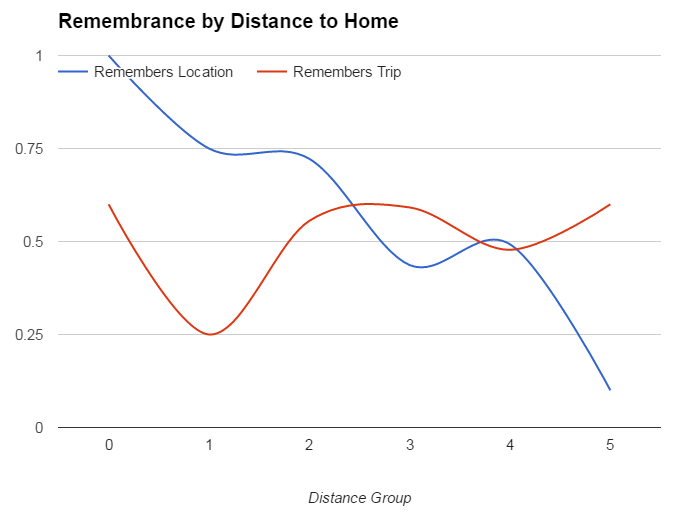
\includegraphics[width=1\linewidth]{distance}
% 	\caption{Location remembrance is inversely correlated to its distance from a participant's home.}
% 	\label{fig:distancememory}
% \end{figure}

\subsubsection{Visit Frequency}
% only affect location rememberance
% trip rememberance $\chi^2(1,126) = 0.066$, p = 0.3987 (> 0.05)
% most frequently visited - 72%, least frequently visited - 36%, $\chi^2(1,128) = 14.458$, p < 0.01
Location memorability and trip memorability are affected differently by frequency of visits (Figure~\ref{fig:frequencymemory}). Location memorability is highest for places that are most frequently visited by the participant, while trip memorability is highest for places that are least frequently visited. The more frequently a place was visited, the more likely it was that the participant remembered the location when it was shown to them at the study. In the most frequently visited places, participants remembered the location 72\% of the time, while only remembering the location 36\% of the time in least frequently visited places, with a significance at $\chi^2(1,128) = 14.458$, p < 0.01. This effect does not occur for trip memorability. In the most frequently visited places, trips are remembered 51\% of the time. Instead of seeing trip memorability decrease for least frequently visited places, this factor increases to 56\%.

% \begin{figure}
%    \centering
%      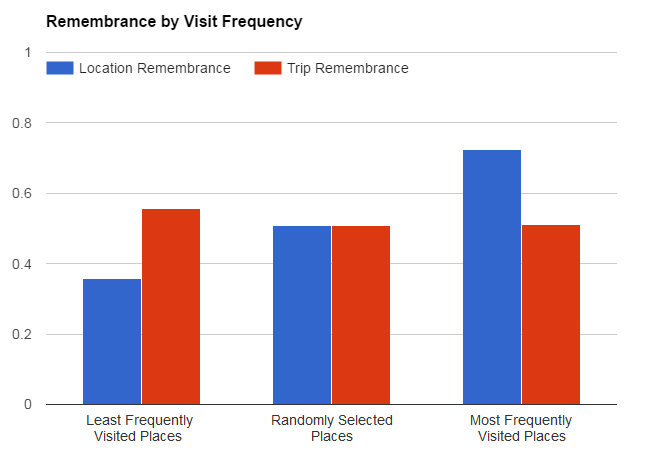
\includegraphics[width=1\linewidth]{RML_2}
%      \caption{Locations were more likely to be remembered where participants had visited the place more, whereas trips were more likely to be remembered where participants had visited the place less.}
%      \label{fig:frequencymemory}
% \end{figure}



% \begin{figure}
% 	\centering
% 	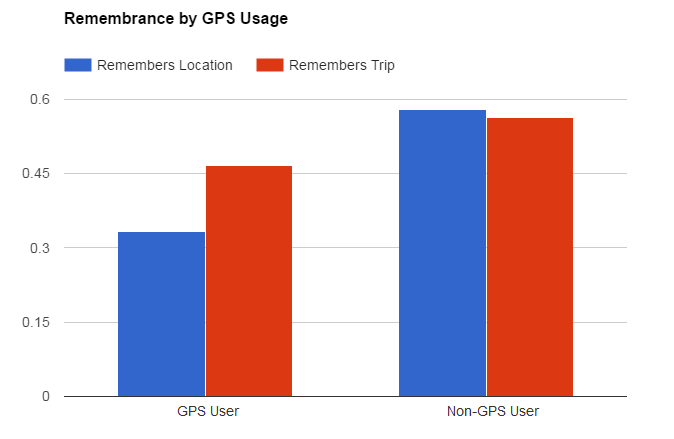
\includegraphics[width=1\linewidth]{GPS_remembrance_2}
% 	\caption{Regular GPS users remembered locations 33\% of the time and trips 47\%, compared to 58\% and 56\% for non-regular GPS users.}
% 	\label{fig:gpsmemory}
% \end{figure}


\subsubsection{Other Variables}
% needs to be filled?

\subsection{Believability}
Rewinds should be believable as memories, and be able to serve as digitally-sourced memories of locations and trips. For that purpose, we define the believability of a Rewind as its accuracy to the participant's memories. Here we will look at how GPS usage and visit frequency affect participants' believability judgments, and discuss the features that participants pointed out as either contributing to or detracting from a Rewind's believability.

\subsubsection{GPS Usage}
% no significant effects on location belivability $\chi^2(1,86) = 0.666$, p = 0.2073(> 0.05)
% signifant effects on trip belivability $\chi^2(1,128) = 2.917$, p = 0.0483(< 0.05)
% GPS - 69%, non-GPS - 81%
Our results show that participants who were non-regular GPS users found photos and Rewinds to be accurate to their memory more often than regular GPS users did. Photos and Rewinds could only be considered accurate to a participant's memory if the participant first confirmed that they remembered the locations in them. The results in this section reflect percentages from a total pool of only photos and Rewinds that have remembered locations. Regular GPS users found 65\% of photos and 45\% of Rewinds accurate to their memory out of the photos and Rewinds in which they remembered the locations. Participants who did not regularly use GPS found 78\% of photos and 63\% of Rewinds accurate to their memory. So far, our findings show that regular GPS users remembered the locations in their digital memories less often, and from the locations they did remember, they were less likely to find a photo or Rewind accurate to their memory. One participant who identified as a regular GPS user said, ``I really don't pay attention to my surroundings when I'm driving. I'm focused on the GPS and the road,'' when asked about the accuracy of a trip.


\subsubsection{Frequent Travelers}
% no significant effects on photo belivability $\chi^2(1,86) = 0$, p = 0.4947(> 0.05)
% significant effects on video belivability $\chi^2(1,128) = 5.837$, p = 0.0079 (< 0.01)
% frequent - 86%, non-frequent - 65%



\subsubsection{Travel Companions}
% significant effects on photo/location belivability $\chi^2(1,91) = 20.956$, p < 0.01
% traveling alone - 82%, not alone - 25%
% significant effects on video/trip belivability if we use alpha = 0.1 - $\chi^2(1,127) = 1.865$, p = 0.086(< 0.1)
% traveling alone - 84%, not alone - 72%
Whether or not the participant was traveling alone during a trip is a significant predictor for whether the trip's associated Rewind will be kept. Rewinds in which the participant is traveling with another person make up about a fifth of all Rewinds in the entire study, but make up over half of the Rewinds that participants actually want to keep. Of Rewinds that participants judged desirable enough to keep, 39\% of were of trips in which the participant is traveling alone, and 54\% are of trips in which the participant is traveling with others. The data shows clearly that a Rewind is considered more valuable if the trip it depicts was taken with company. 


\subsubsection{Distance}
% no ignificant effects on photo/location belivability $\chi^2(5,86) = 7.745$, p = 0.1709 (> 0.05)
% significant effects on video/trip belivability if we use alpha = 0.1 - $\chi^2(5,128) = 10.093$, p = 0.0726(< 0.1)
% 0 - 100%, 1 - 75%, 2 - 75%, 3 - 85%, 4 - 80%, 5 - 33%


\subsubsection{Visit Frequency}
% significant effects on photo belivability if we use alpha = 0.1 - $\chi^2(1,61) = 2.012$, p = 0.078(< 0.1)
% most frequently visited location - 71%, least frequently visited location - 89%
% no significant effects on video/trip belivability $\chi^2(1,91) = 0.951$, p = 0.1647(> 0.05)
% trip that include most frequently visited locations  -  70%, trip that include least frequently visited locations - 81%
We found that the more visits a location had, the less likely it was for the Rewind associated with it to be judged as accurate by the participant. Trips with a location that was visited most frequently by the participant were said to be accurate 75\% of the time. The more a person visits a location, the more they may notice inconsistencies between the actual place and a digitally-fabricated memory of it. Trips with a location that was visited least frequently had a higher accuracy rating of 82\%.

% (Jeff): this figure is probably best replaced with some text
%\begin{figure}
%   \centering
%     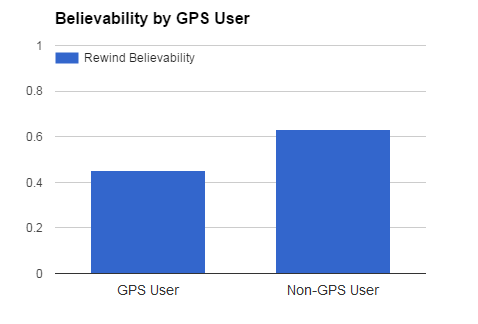
\includegraphics[width=1\linewidth]{GPS_believability_2}
%     \caption{Participants who did not use GPS regularly found Rewinds to be accurate to their memory more often than regular GPS users did.}
%     \label{scroll}
%\end{figure}

\subsection{Desirability}
For Rewinds to be useful, they need to have value to their owners. We measured the value of photos and Rewinds by asking participants if they would want to keep the photo or Rewind after seeing it. Overall, participants wished to keep 11\% of the photos they were shown and 15\% of the Rewinds they were shown. Because these were images from third-party services, they are naturally less likely to be desirable than media captured by the user themselves. In this section we will look at how the value of Rewind's digitally-fabricated memories differs between participants who consider themselves frequent travelers and participants who don't. We will also examine how visit frequency and travel companionship affect the desirability of a Rewind.

\subsubsection{GPS usage}
% no significant effects on photo desirability $\chi^2(1,179) = 0.338$, p = 0.2804(> 0.05)
% significant effects on video/trip desirability $\chi^2(1, 177) = 7.319$, p = 0.0034(< 0.01)
% GPS - 26%, non-GPS - 9%

\subsection{Frequent Travellers}
% no significant effects on photo desirability $\chi^2(1,179) = 0.828$, p = 0.1814(> 0.05)
% significant effects on video/trip desirability $\chi^2(1, 179) = 9.754$, p = 0.0009(< 0.01)
% frequent - 21 %, non-frequent - 2%
Our study found that participants who considered themselves frequent travelers were more likely to keep their photos and Rewinds than participants who did not identify as frequent travelers. Frequent travelers kept 13\% of the photos they were shown and 21\% of Rewinds. But participants who identified as infrequent travelers kept only 7\% of photos and 2\% of Rewinds. The results show that those who consider themselves frequent travelers tend to place higher value on digital memories than those who do not identify as frequent travelers.

\subsubsection{Travel Companions}
% no significant effects on photo desirability $\chi^2(1,94) = 0.071$, p = 0.3948(> 0.05)
% significant effects on video/trip desirability if alpha = 0.1 - $\chi^2(1, 133) = 2.443$, p = 0.059(< 0.1)
% alone - 13%, not alone - 26%

\subsubsection{Distance}
% no significant effects on photo desirability $\chi^2(1,179) = 8.131$, p = 0.1492(> 0.05)
% significant effects on video/trip desirability if alphe = 0.1 -  $\chi^2(5, 177) = 10.084$, p = 0.0729(< 0.1)
% 0 - 0%, 1 - 0%, 2 - 11%,  3 - 10%, 4 - 20%,  5 - 40% 

\subsubsection{Visit Frequency}
% no significant effects on photo desirability $\chi^2(1,128) = 0.32$, p = 0.2858(> 0.05)
% most - 15%, least - 10%
%  no significant effects on video/trip desirability $\chi^2(1, 126) = 0.552$, p = 0.2288(> 0.05)
% most - 11%, least - 18%
We found that the desirability of a Rewind is partly influenced by how much the participant visits the location associated with the Rewind. Rewinds containing a location visited most frequently by the participant are kept 8\% of the time. This percentage increases significantly if the Rewind contains the location visited least frequently by the participant. Rewinds that include the least visited location are kept 13\% of the time. This data suggests that Rewinds are more desirable if they portray a trip that has locations that are not visited often.


\subsubsection{Features}
To get a better understanding of what the important features of locational memories are, we looked at participants' responses to why they thought a Rewind was or was not accurate to their memory. Participants attributed the accuracy of a Rewind to the presence of different man-made structures. The most highly occurring answers to why a Rewind was accurate were: the route, the highways, roads, and streets, the signs, the landmarks, and the buildings. The reasons why a Rewind did not seem accurate to participants' memories included more temporal and environmental features. When participants responded that a Rewind was not accurate to their memory, they cited the streets, the season and foliage, the time of day, and the angle the Rewind viewed the world at as factors of inaccuracy.

Our results show that GPS usage influences what features participants pick out when deciding whether Rewinds are accurate reflections of their own memories of their trips. When we split the responses of regular GPS users from the other participants' responses, we saw that GPS users looked at signs in the Rewind the most to determine accuracy. Participants who were not regular GPS users cited the route and surrounding landmarks as features which made the Rewind believable as memories.




% \begin{figure}
%    \centering
%      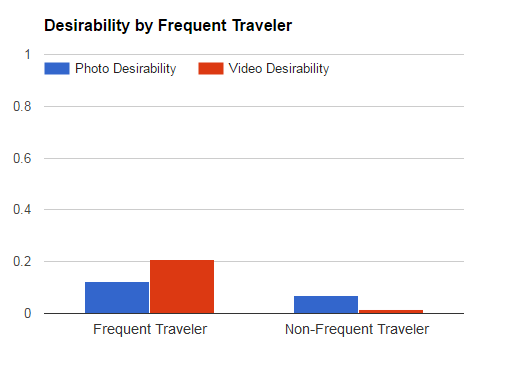
\includegraphics[width=1\linewidth]{FreqTraveler_keep_2}
%      \caption{Frequent travelers are more willing to keep copies of photos and Rewinds.}
%      \label{fig:frequencydesire}
% \end{figure}



\subsubsection{Participant Responses}
When asked why they wanted to keep or not keep a photo or Rewind, patterns emerged in the participants' answers. Participants didn't want to keep anything that was ``no use'' or had ``no meaning or significance.'' One participant said they ``didn't need any more memories of work.'' Some participants acknowledged the ``good composition,'' and one said, ``It's not a bad photo but it wasn't taken by me.'' Participants were most likely to keep photos that reminded them of good memories, 

\subsection{Participant Reactions}
There was a range of behaviors and attitudes toward Rewinds from the participants. One participant called Rewinds ``creepy, eerie,'' and said they might ``show them to a friend who's a conspiracy theorist.'' Another participant proclaimed that they weren't ``paranoid about technology.'' Many participants, especially regular GPS users, examined signs in Rewinds intensely, looking at highway exit signs to try to remember their trip. Other participants did not feel positive after watching their Rewinds, saying that they ``just realized how often [they] take the same route,'' or that they felt like they ``needed to switch up [their] routine.'' One participant was amazed, and exclaimed, ``It's like it's happening!'' But the most important responses were from participants who changed their responses after recognizing an image in their Rewind: ``I recognize the photo now.'' The Rewind had helped them remember the location of the original image.

\section{Discussion}
This work explores a future where digital memories can be retrieved in an instant, regenerated from trace data which is becoming increasingly ubiquitous. The ability to perform these actions encourages humanist values of self-reflection and intentional living. We seek to design an application that can produce moments of delight and thoughtful reflection.

While the study results provide a wealth of correlations between varying factors and participant groups, our most significant findings pertain to the effects of regular GPS usage, visit frequency, and travel companionship on Rewind memorability, believability, and desirability. Regular GPS users are less able to remember locations and trips, and more often rely on road signs to jog their memory or determine Rewind believability. This confirms Leshed et al.'s findings that GPS users are typically disengaged with their environment \cite{leshed2008car}. We found that while GPS users had lower remembrance overall, the group experienced a jump between location remembrance and trip remembrance, suggesting that Rewinds may actually engage GPS users' memories. 

We see high visit frequencies resulting in lower Rewind believability and low visit frequencies making Rewinds more desirable. This is quite intuitive because if you visit a place often, it is harder to distinguish the exact, particular trip you took to that place, just because there are more trips to choose from. Locations that you visit infrequently are likely special occasions, thus making the Rewinds more desirable because they present a precious memory.

Lastly, our results show that Rewinds of trips taken with a companion hold more value and are more memorable to participants. This supports van Dijck's idea that ``recall tends to lean on a sense of belonging or sharing'' \cite{van2007mediated}.

%What applications or tasks are possible now that we have made these discoveries/inventions?
%What can this be used for?
%		Ex: It can help people remember the past
		
%What are some implications for designing systems/interfaces in the future?
%	What would you tell a person who will design a similar system?
%		Ex: Scrolling is important for the user to be able to take a closer look at Rewinds., talk about features for believability

There are some inherent limitations to Rewind due to today's technologies. Location data is imperfect, and often can hop around the map, showing the user places they may have never been. But even more important is the limits to how realistic a Rewind can truly be. People and conversations, which are what we think about often, can't be shown in Rewinds without some additional recording device. Therefore, while Rewind does not recreate the exact memory, it's a proxy for what environment where the memory occurs.

\subsection{Rewinds More Real and More Salient}

How realistic can Rewind become in the near future? Currently, most street side images are of the road, as cameras that take these photos are attached to cars. But other forms of imagery have recently arrived: Google and Bing have expanded their street side photos to inside buildings, on hiking trails, and campus greens, and recent open source street side offerings like OpenStreetView have surfaced. Satellite images can be used for travel in airplanes and simulate the view outside the window from seat 17F. More sophisticated image manipulation algorithms are already here, but take many minutes to run offline (e.g., \cite{laffont2014transient,shih2013data}). Eventually, as computing performance continues to improve, and further research is done on the software, it's likely that entire Rewinds can be adjusted in real-time.

Besides visuals, a salient part of a memory is in the sounds from the past. This can be replicated through a number of styles: the pitter-patter of footsteps or sound of driving through the streets (mode of transportation can be detected purely from geolocation data \cite{zheng2008learning}), the whistle of the winds or thunderstorms at night, and even sounds based on geographical features like when the user was near water or by a outdoor market. van Dijck explains, ``One memory rarely encompasses all sensory modes, because we tend to remember by selecting particular ones. For instance, we may recall a mood, locale or era through a particular smell (such as the smell of apple pie in the oven triggering the image of your mother's kitchen on Saturday afternoons), or we may remember a person by his nasal voice or twinkling eyes'' \cite{van2007mediated} (pg. 20). Audio and visuals combined can enrich the experience, as Rewind uses environmental data such as weather information or the season to incorporate other sensory modes. By leveraging environmental sensory data, users may be stimulated to recall something that may have been forgotten otherwise, and this information makes the experience feel more real.

In another direction, Rewind can be applied to virtual reality environments. Besides the visual and audio immersion, in a virtual reality environment, the user is physically situated inside the environment. Rather than sitting in a chair looking at a screen, the user is standing where they would have been standing in the past. This changes the experience from ``watching'' to ``being'' present in the past. Virtual reality environments have already been used as a tool to study human memory \cite{gamberini2000virtual}, so it is a natural extension for Rewind. To stand there with the power to scrub back and forth in time could create a new mode for experiencing memories.

One of the applications of Rewind is to support people with memory loss, those who have Alzheimer's or short-term amnesia. For example, photographs have been known to stimulate the memory of people afflicted with Alzheimer's \cite{grandmaison2003critical}. To be able to do the same, but with a sequence of realistic audio-visuals, may turn something that was forgotten back into a memory, and doing so for an important place or trip would be exciting.

\section{Conclusion}
We forget so much. So our own memories are incomplete glimpses of the past. Yet they are part of who we are. The ultimate goal of the Rewind system is to envision a new way to digitally capture memories in the future. As there are an increasing number of sensors (cameras, weather, microphones) in the environment, being able to reconstruct a rich experience becomes more feasible. Personal reflection and recalling the past has significance for everyone. A new form of digital memories is a direct tangible benefit people can get from their user own personal informatics data, and one that they have full control over.

Our study of people using Rewinds over 2 weeks reveals some interesting findings. When people are shown just a photograph, they remember the location half the time; but when shown a Rewind, participants nearly always remembered the location. We find that people who commonly use GPS devices do not remember places as well; they seem to notice street signs, routes, and landmarks more so than those who do not. When Rewinds are inaccurate, it's from people noticing the wrong season, view angle, or time of day. These are challenges that we are facing but trying to address through image manipulation based on past data. And we find that people are more likely to remember places that they visit more frequently, as expected. Rewinds are not really for places that you go often, as for those, the location is more memorable as a photo. But infrequent trips are where Rewinds can help someone resurface a memory, and take you back to the road less traveled.

\section{Acknowledgments}
[anonymized for review]

\balance

\bibliographystyle{SIGCHI-Reference-Format}
\bibliography{paper}
\end{document}
